
    




    
\documentclass[10pt,notitlepage,onecolumn,aps,pra]{revtex4-1}

    
    
\usepackage[T1]{fontenc}
\usepackage{graphicx}
% We will generate all images so they have a width \maxwidth. This means
% that they will get their normal width if they fit onto the page, but
% are scaled down if they would overflow the margins.
\makeatletter
\def\maxwidth{\ifdim\Gin@nat@width>\linewidth\linewidth
\else\Gin@nat@width\fi}
\makeatother
\let\Oldincludegraphics\includegraphics
% Set max figure width to be 80% of text width, for now hardcoded.
\renewcommand{\includegraphics}[1]{\Oldincludegraphics[width=.8\maxwidth]{#1}}
% Ensure that by default, figures have no caption (until we provide a
% proper Figure object with a Caption API and a way to capture that
% in the conversion process - todo).
\usepackage{caption}
\DeclareCaptionLabelFormat{nolabel}{}
\captionsetup{labelformat=nolabel}

\usepackage{adjustbox} % Used to constrain images to a maximum size
\usepackage{xcolor} % Allow colors to be defined
\usepackage{enumerate} % Needed for markdown enumerations to work
\usepackage{geometry} % Used to adjust the document margins
\usepackage{amsmath} % Equations
\usepackage{amssymb} % Equations
\usepackage{textcomp} % defines textquotesingle
% Hack from http://tex.stackexchange.com/a/47451/13684:
\AtBeginDocument{%
    \def\PYZsq{\textquotesingle}% Upright quotes in Pygmentized code
}
\usepackage{upquote} % Upright quotes for verbatim code
\usepackage{eurosym} % defines \euro
\usepackage[mathletters]{ucs} % Extended unicode (utf-8) support
\usepackage[utf8x]{inputenc} % Allow utf-8 characters in the tex document
\usepackage{fancyvrb} % verbatim replacement that allows latex
\usepackage{grffile} % extends the file name processing of package graphics
                     % to support a larger range
% The hyperref package gives us a pdf with properly built
% internal navigation ('pdf bookmarks' for the table of contents,
% internal cross-reference links, web links for URLs, etc.)
\usepackage{hyperref}
\usepackage{booktabs}  % table support for pandoc > 1.12.2
\usepackage[inline]{enumitem} % IRkernel/repr support (it uses the enumerate* environment)
\usepackage[normalem]{ulem} % ulem is needed to support strikethroughs (\sout)
                            % normalem makes italics be italics, not underlines
\usepackage{braket}


    
    % Colors for the hyperref package
    \definecolor{urlcolor}{rgb}{0,.145,.698}
    \definecolor{linkcolor}{rgb}{.71,0.21,0.01}
    \definecolor{citecolor}{rgb}{.12,.54,.11}

    % ANSI colors
    \definecolor{ansi-black}{HTML}{3E424D}
    \definecolor{ansi-black-intense}{HTML}{282C36}
    \definecolor{ansi-red}{HTML}{E75C58}
    \definecolor{ansi-red-intense}{HTML}{B22B31}
    \definecolor{ansi-green}{HTML}{00A250}
    \definecolor{ansi-green-intense}{HTML}{007427}
    \definecolor{ansi-yellow}{HTML}{DDB62B}
    \definecolor{ansi-yellow-intense}{HTML}{B27D12}
    \definecolor{ansi-blue}{HTML}{208FFB}
    \definecolor{ansi-blue-intense}{HTML}{0065CA}
    \definecolor{ansi-magenta}{HTML}{D160C4}
    \definecolor{ansi-magenta-intense}{HTML}{A03196}
    \definecolor{ansi-cyan}{HTML}{60C6C8}
    \definecolor{ansi-cyan-intense}{HTML}{258F8F}
    \definecolor{ansi-white}{HTML}{C5C1B4}
    \definecolor{ansi-white-intense}{HTML}{A1A6B2}
    \definecolor{ansi-default-inverse-fg}{HTML}{FFFFFF}
    \definecolor{ansi-default-inverse-bg}{HTML}{000000}

    % commands and environments needed by pandoc snippets
    % extracted from the output of `pandoc -s`
    \providecommand{\tightlist}{%
      \setlength{\itemsep}{0pt}\setlength{\parskip}{0pt}}
    \DefineVerbatimEnvironment{Highlighting}{Verbatim}{commandchars=\\\{\}}
    % Add ',fontsize=\small' for more characters per line
    \newenvironment{Shaded}{}{}
    \newcommand{\KeywordTok}[1]{\textcolor[rgb]{0.00,0.44,0.13}{\textbf{{#1}}}}
    \newcommand{\DataTypeTok}[1]{\textcolor[rgb]{0.56,0.13,0.00}{{#1}}}
    \newcommand{\DecValTok}[1]{\textcolor[rgb]{0.25,0.63,0.44}{{#1}}}
    \newcommand{\BaseNTok}[1]{\textcolor[rgb]{0.25,0.63,0.44}{{#1}}}
    \newcommand{\FloatTok}[1]{\textcolor[rgb]{0.25,0.63,0.44}{{#1}}}
    \newcommand{\CharTok}[1]{\textcolor[rgb]{0.25,0.44,0.63}{{#1}}}
    \newcommand{\StringTok}[1]{\textcolor[rgb]{0.25,0.44,0.63}{{#1}}}
    \newcommand{\CommentTok}[1]{\textcolor[rgb]{0.38,0.63,0.69}{\textit{{#1}}}}
    \newcommand{\OtherTok}[1]{\textcolor[rgb]{0.00,0.44,0.13}{{#1}}}
    \newcommand{\AlertTok}[1]{\textcolor[rgb]{1.00,0.00,0.00}{\textbf{{#1}}}}
    \newcommand{\FunctionTok}[1]{\textcolor[rgb]{0.02,0.16,0.49}{{#1}}}
    \newcommand{\RegionMarkerTok}[1]{{#1}}
    \newcommand{\ErrorTok}[1]{\textcolor[rgb]{1.00,0.00,0.00}{\textbf{{#1}}}}
    \newcommand{\NormalTok}[1]{{#1}}
    
    % Additional commands for more recent versions of Pandoc
    \newcommand{\ConstantTok}[1]{\textcolor[rgb]{0.53,0.00,0.00}{{#1}}}
    \newcommand{\SpecialCharTok}[1]{\textcolor[rgb]{0.25,0.44,0.63}{{#1}}}
    \newcommand{\VerbatimStringTok}[1]{\textcolor[rgb]{0.25,0.44,0.63}{{#1}}}
    \newcommand{\SpecialStringTok}[1]{\textcolor[rgb]{0.73,0.40,0.53}{{#1}}}
    \newcommand{\ImportTok}[1]{{#1}}
    \newcommand{\DocumentationTok}[1]{\textcolor[rgb]{0.73,0.13,0.13}{\textit{{#1}}}}
    \newcommand{\AnnotationTok}[1]{\textcolor[rgb]{0.38,0.63,0.69}{\textbf{\textit{{#1}}}}}
    \newcommand{\CommentVarTok}[1]{\textcolor[rgb]{0.38,0.63,0.69}{\textbf{\textit{{#1}}}}}
    \newcommand{\VariableTok}[1]{\textcolor[rgb]{0.10,0.09,0.49}{{#1}}}
    \newcommand{\ControlFlowTok}[1]{\textcolor[rgb]{0.00,0.44,0.13}{\textbf{{#1}}}}
    \newcommand{\OperatorTok}[1]{\textcolor[rgb]{0.40,0.40,0.40}{{#1}}}
    \newcommand{\BuiltInTok}[1]{{#1}}
    \newcommand{\ExtensionTok}[1]{{#1}}
    \newcommand{\PreprocessorTok}[1]{\textcolor[rgb]{0.74,0.48,0.00}{{#1}}}
    \newcommand{\AttributeTok}[1]{\textcolor[rgb]{0.49,0.56,0.16}{{#1}}}
    \newcommand{\InformationTok}[1]{\textcolor[rgb]{0.38,0.63,0.69}{\textbf{\textit{{#1}}}}}
    \newcommand{\WarningTok}[1]{\textcolor[rgb]{0.38,0.63,0.69}{\textbf{\textit{{#1}}}}}
    
    
    % Define a nice break command that doesn't care if a line doesn't already
    % exist.
    \def\br{\hspace*{\fill} \\* }
    % Math Jax compatibility definitions
    \def\gt{>}
    \def\lt{<}
    \let\Oldtex\TeX
    \let\Oldlatex\LaTeX
    \renewcommand{\TeX}{\textrm{\Oldtex}}
    \renewcommand{\LaTeX}{\textrm{\Oldlatex}}
    % Document parameters
    % Document title
    
    
    
    
% Pygments definitions
\makeatletter
\def\PY@reset{\let\PY@it=\relax \let\PY@bf=\relax%
    \let\PY@ul=\relax \let\PY@tc=\relax%
    \let\PY@bc=\relax \let\PY@ff=\relax}
\def\PY@tok#1{\csname PY@tok@#1\endcsname}
\def\PY@toks#1+{\ifx\relax#1\empty\else%
    \PY@tok{#1}\expandafter\PY@toks\fi}
\def\PY@do#1{\PY@bc{\PY@tc{\PY@ul{%
    \PY@it{\PY@bf{\PY@ff{#1}}}}}}}
\def\PY#1#2{\PY@reset\PY@toks#1+\relax+\PY@do{#2}}

\expandafter\def\csname PY@tok@w\endcsname{\def\PY@tc##1{\textcolor[rgb]{0.73,0.73,0.73}{##1}}}
\expandafter\def\csname PY@tok@c\endcsname{\let\PY@it=\textit\def\PY@tc##1{\textcolor[rgb]{0.25,0.50,0.50}{##1}}}
\expandafter\def\csname PY@tok@cp\endcsname{\def\PY@tc##1{\textcolor[rgb]{0.74,0.48,0.00}{##1}}}
\expandafter\def\csname PY@tok@k\endcsname{\let\PY@bf=\textbf\def\PY@tc##1{\textcolor[rgb]{0.00,0.50,0.00}{##1}}}
\expandafter\def\csname PY@tok@kp\endcsname{\def\PY@tc##1{\textcolor[rgb]{0.00,0.50,0.00}{##1}}}
\expandafter\def\csname PY@tok@kt\endcsname{\def\PY@tc##1{\textcolor[rgb]{0.69,0.00,0.25}{##1}}}
\expandafter\def\csname PY@tok@o\endcsname{\def\PY@tc##1{\textcolor[rgb]{0.40,0.40,0.40}{##1}}}
\expandafter\def\csname PY@tok@ow\endcsname{\let\PY@bf=\textbf\def\PY@tc##1{\textcolor[rgb]{0.67,0.13,1.00}{##1}}}
\expandafter\def\csname PY@tok@nb\endcsname{\def\PY@tc##1{\textcolor[rgb]{0.00,0.50,0.00}{##1}}}
\expandafter\def\csname PY@tok@nf\endcsname{\def\PY@tc##1{\textcolor[rgb]{0.00,0.00,1.00}{##1}}}
\expandafter\def\csname PY@tok@nc\endcsname{\let\PY@bf=\textbf\def\PY@tc##1{\textcolor[rgb]{0.00,0.00,1.00}{##1}}}
\expandafter\def\csname PY@tok@nn\endcsname{\let\PY@bf=\textbf\def\PY@tc##1{\textcolor[rgb]{0.00,0.00,1.00}{##1}}}
\expandafter\def\csname PY@tok@ne\endcsname{\let\PY@bf=\textbf\def\PY@tc##1{\textcolor[rgb]{0.82,0.25,0.23}{##1}}}
\expandafter\def\csname PY@tok@nv\endcsname{\def\PY@tc##1{\textcolor[rgb]{0.10,0.09,0.49}{##1}}}
\expandafter\def\csname PY@tok@no\endcsname{\def\PY@tc##1{\textcolor[rgb]{0.53,0.00,0.00}{##1}}}
\expandafter\def\csname PY@tok@nl\endcsname{\def\PY@tc##1{\textcolor[rgb]{0.63,0.63,0.00}{##1}}}
\expandafter\def\csname PY@tok@ni\endcsname{\let\PY@bf=\textbf\def\PY@tc##1{\textcolor[rgb]{0.60,0.60,0.60}{##1}}}
\expandafter\def\csname PY@tok@na\endcsname{\def\PY@tc##1{\textcolor[rgb]{0.49,0.56,0.16}{##1}}}
\expandafter\def\csname PY@tok@nt\endcsname{\let\PY@bf=\textbf\def\PY@tc##1{\textcolor[rgb]{0.00,0.50,0.00}{##1}}}
\expandafter\def\csname PY@tok@nd\endcsname{\def\PY@tc##1{\textcolor[rgb]{0.67,0.13,1.00}{##1}}}
\expandafter\def\csname PY@tok@s\endcsname{\def\PY@tc##1{\textcolor[rgb]{0.73,0.13,0.13}{##1}}}
\expandafter\def\csname PY@tok@sd\endcsname{\let\PY@it=\textit\def\PY@tc##1{\textcolor[rgb]{0.73,0.13,0.13}{##1}}}
\expandafter\def\csname PY@tok@si\endcsname{\let\PY@bf=\textbf\def\PY@tc##1{\textcolor[rgb]{0.73,0.40,0.53}{##1}}}
\expandafter\def\csname PY@tok@se\endcsname{\let\PY@bf=\textbf\def\PY@tc##1{\textcolor[rgb]{0.73,0.40,0.13}{##1}}}
\expandafter\def\csname PY@tok@sr\endcsname{\def\PY@tc##1{\textcolor[rgb]{0.73,0.40,0.53}{##1}}}
\expandafter\def\csname PY@tok@ss\endcsname{\def\PY@tc##1{\textcolor[rgb]{0.10,0.09,0.49}{##1}}}
\expandafter\def\csname PY@tok@sx\endcsname{\def\PY@tc##1{\textcolor[rgb]{0.00,0.50,0.00}{##1}}}
\expandafter\def\csname PY@tok@m\endcsname{\def\PY@tc##1{\textcolor[rgb]{0.40,0.40,0.40}{##1}}}
\expandafter\def\csname PY@tok@gh\endcsname{\let\PY@bf=\textbf\def\PY@tc##1{\textcolor[rgb]{0.00,0.00,0.50}{##1}}}
\expandafter\def\csname PY@tok@gu\endcsname{\let\PY@bf=\textbf\def\PY@tc##1{\textcolor[rgb]{0.50,0.00,0.50}{##1}}}
\expandafter\def\csname PY@tok@gd\endcsname{\def\PY@tc##1{\textcolor[rgb]{0.63,0.00,0.00}{##1}}}
\expandafter\def\csname PY@tok@gi\endcsname{\def\PY@tc##1{\textcolor[rgb]{0.00,0.63,0.00}{##1}}}
\expandafter\def\csname PY@tok@gr\endcsname{\def\PY@tc##1{\textcolor[rgb]{1.00,0.00,0.00}{##1}}}
\expandafter\def\csname PY@tok@ge\endcsname{\let\PY@it=\textit}
\expandafter\def\csname PY@tok@gs\endcsname{\let\PY@bf=\textbf}
\expandafter\def\csname PY@tok@gp\endcsname{\let\PY@bf=\textbf\def\PY@tc##1{\textcolor[rgb]{0.00,0.00,0.50}{##1}}}
\expandafter\def\csname PY@tok@go\endcsname{\def\PY@tc##1{\textcolor[rgb]{0.53,0.53,0.53}{##1}}}
\expandafter\def\csname PY@tok@gt\endcsname{\def\PY@tc##1{\textcolor[rgb]{0.00,0.27,0.87}{##1}}}
\expandafter\def\csname PY@tok@err\endcsname{\def\PY@bc##1{\setlength{\fboxsep}{0pt}\fcolorbox[rgb]{1.00,0.00,0.00}{1,1,1}{\strut ##1}}}
\expandafter\def\csname PY@tok@kc\endcsname{\let\PY@bf=\textbf\def\PY@tc##1{\textcolor[rgb]{0.00,0.50,0.00}{##1}}}
\expandafter\def\csname PY@tok@kd\endcsname{\let\PY@bf=\textbf\def\PY@tc##1{\textcolor[rgb]{0.00,0.50,0.00}{##1}}}
\expandafter\def\csname PY@tok@kn\endcsname{\let\PY@bf=\textbf\def\PY@tc##1{\textcolor[rgb]{0.00,0.50,0.00}{##1}}}
\expandafter\def\csname PY@tok@kr\endcsname{\let\PY@bf=\textbf\def\PY@tc##1{\textcolor[rgb]{0.00,0.50,0.00}{##1}}}
\expandafter\def\csname PY@tok@bp\endcsname{\def\PY@tc##1{\textcolor[rgb]{0.00,0.50,0.00}{##1}}}
\expandafter\def\csname PY@tok@fm\endcsname{\def\PY@tc##1{\textcolor[rgb]{0.00,0.00,1.00}{##1}}}
\expandafter\def\csname PY@tok@vc\endcsname{\def\PY@tc##1{\textcolor[rgb]{0.10,0.09,0.49}{##1}}}
\expandafter\def\csname PY@tok@vg\endcsname{\def\PY@tc##1{\textcolor[rgb]{0.10,0.09,0.49}{##1}}}
\expandafter\def\csname PY@tok@vi\endcsname{\def\PY@tc##1{\textcolor[rgb]{0.10,0.09,0.49}{##1}}}
\expandafter\def\csname PY@tok@vm\endcsname{\def\PY@tc##1{\textcolor[rgb]{0.10,0.09,0.49}{##1}}}
\expandafter\def\csname PY@tok@sa\endcsname{\def\PY@tc##1{\textcolor[rgb]{0.73,0.13,0.13}{##1}}}
\expandafter\def\csname PY@tok@sb\endcsname{\def\PY@tc##1{\textcolor[rgb]{0.73,0.13,0.13}{##1}}}
\expandafter\def\csname PY@tok@sc\endcsname{\def\PY@tc##1{\textcolor[rgb]{0.73,0.13,0.13}{##1}}}
\expandafter\def\csname PY@tok@dl\endcsname{\def\PY@tc##1{\textcolor[rgb]{0.73,0.13,0.13}{##1}}}
\expandafter\def\csname PY@tok@s2\endcsname{\def\PY@tc##1{\textcolor[rgb]{0.73,0.13,0.13}{##1}}}
\expandafter\def\csname PY@tok@sh\endcsname{\def\PY@tc##1{\textcolor[rgb]{0.73,0.13,0.13}{##1}}}
\expandafter\def\csname PY@tok@s1\endcsname{\def\PY@tc##1{\textcolor[rgb]{0.73,0.13,0.13}{##1}}}
\expandafter\def\csname PY@tok@mb\endcsname{\def\PY@tc##1{\textcolor[rgb]{0.40,0.40,0.40}{##1}}}
\expandafter\def\csname PY@tok@mf\endcsname{\def\PY@tc##1{\textcolor[rgb]{0.40,0.40,0.40}{##1}}}
\expandafter\def\csname PY@tok@mh\endcsname{\def\PY@tc##1{\textcolor[rgb]{0.40,0.40,0.40}{##1}}}
\expandafter\def\csname PY@tok@mi\endcsname{\def\PY@tc##1{\textcolor[rgb]{0.40,0.40,0.40}{##1}}}
\expandafter\def\csname PY@tok@il\endcsname{\def\PY@tc##1{\textcolor[rgb]{0.40,0.40,0.40}{##1}}}
\expandafter\def\csname PY@tok@mo\endcsname{\def\PY@tc##1{\textcolor[rgb]{0.40,0.40,0.40}{##1}}}
\expandafter\def\csname PY@tok@ch\endcsname{\let\PY@it=\textit\def\PY@tc##1{\textcolor[rgb]{0.25,0.50,0.50}{##1}}}
\expandafter\def\csname PY@tok@cm\endcsname{\let\PY@it=\textit\def\PY@tc##1{\textcolor[rgb]{0.25,0.50,0.50}{##1}}}
\expandafter\def\csname PY@tok@cpf\endcsname{\let\PY@it=\textit\def\PY@tc##1{\textcolor[rgb]{0.25,0.50,0.50}{##1}}}
\expandafter\def\csname PY@tok@c1\endcsname{\let\PY@it=\textit\def\PY@tc##1{\textcolor[rgb]{0.25,0.50,0.50}{##1}}}
\expandafter\def\csname PY@tok@cs\endcsname{\let\PY@it=\textit\def\PY@tc##1{\textcolor[rgb]{0.25,0.50,0.50}{##1}}}

\def\PYZbs{\char`\\}
\def\PYZus{\char`\_}
\def\PYZob{\char`\{}
\def\PYZcb{\char`\}}
\def\PYZca{\char`\^}
\def\PYZam{\char`\&}
\def\PYZlt{\char`\<}
\def\PYZgt{\char`\>}
\def\PYZsh{\char`\#}
\def\PYZpc{\char`\%}
\def\PYZdl{\char`\$}
\def\PYZhy{\char`\-}
\def\PYZsq{\char`\'}
\def\PYZdq{\char`\"}
\def\PYZti{\char`\~}
% for compatibility with earlier versions
\def\PYZat{@}
\def\PYZlb{[}
\def\PYZrb{]}
\makeatother


    % For linebreaks inside Verbatim environment from package fancyvrb. 
    \makeatletter
        \newbox\Wrappedcontinuationbox 
        \newbox\Wrappedvisiblespacebox 
        \newcommand*\Wrappedvisiblespace {\textcolor{red}{\textvisiblespace}} 
        \newcommand*\Wrappedcontinuationsymbol {\textcolor{red}{\llap{\tiny$\m@th\hookrightarrow$}}} 
        \newcommand*\Wrappedcontinuationindent {3ex } 
        \newcommand*\Wrappedafterbreak {\kern\Wrappedcontinuationindent\copy\Wrappedcontinuationbox} 
        % Take advantage of the already applied Pygments mark-up to insert 
        % potential linebreaks for TeX processing. 
        %        {, <, #, %, $, ' and ": go to next line. 
        %        _, }, ^, &, >, - and ~: stay at end of broken line. 
        % Use of \textquotesingle for straight quote. 
        \newcommand*\Wrappedbreaksatspecials {% 
            \def\PYGZus{\discretionary{\char`\_}{\Wrappedafterbreak}{\char`\_}}% 
            \def\PYGZob{\discretionary{}{\Wrappedafterbreak\char`\{}{\char`\{}}% 
            \def\PYGZcb{\discretionary{\char`\}}{\Wrappedafterbreak}{\char`\}}}% 
            \def\PYGZca{\discretionary{\char`\^}{\Wrappedafterbreak}{\char`\^}}% 
            \def\PYGZam{\discretionary{\char`\&}{\Wrappedafterbreak}{\char`\&}}% 
            \def\PYGZlt{\discretionary{}{\Wrappedafterbreak\char`\<}{\char`\<}}% 
            \def\PYGZgt{\discretionary{\char`\>}{\Wrappedafterbreak}{\char`\>}}% 
            \def\PYGZsh{\discretionary{}{\Wrappedafterbreak\char`\#}{\char`\#}}% 
            \def\PYGZpc{\discretionary{}{\Wrappedafterbreak\char`\%}{\char`\%}}% 
            \def\PYGZdl{\discretionary{}{\Wrappedafterbreak\char`\$}{\char`\$}}% 
            \def\PYGZhy{\discretionary{\char`\-}{\Wrappedafterbreak}{\char`\-}}% 
            \def\PYGZsq{\discretionary{}{\Wrappedafterbreak\textquotesingle}{\textquotesingle}}% 
            \def\PYGZdq{\discretionary{}{\Wrappedafterbreak\char`\"}{\char`\"}}% 
            \def\PYGZti{\discretionary{\char`\~}{\Wrappedafterbreak}{\char`\~}}% 
        } 
        % Some characters . , ; ? ! / are not pygmentized. 
        % This macro makes them "active" and they will insert potential linebreaks 
        \newcommand*\Wrappedbreaksatpunct {% 
            \lccode`\~`\.\lowercase{\def~}{\discretionary{\hbox{\char`\.}}{\Wrappedafterbreak}{\hbox{\char`\.}}}% 
            \lccode`\~`\,\lowercase{\def~}{\discretionary{\hbox{\char`\,}}{\Wrappedafterbreak}{\hbox{\char`\,}}}% 
            \lccode`\~`\;\lowercase{\def~}{\discretionary{\hbox{\char`\;}}{\Wrappedafterbreak}{\hbox{\char`\;}}}% 
            \lccode`\~`\:\lowercase{\def~}{\discretionary{\hbox{\char`\:}}{\Wrappedafterbreak}{\hbox{\char`\:}}}% 
            \lccode`\~`\?\lowercase{\def~}{\discretionary{\hbox{\char`\?}}{\Wrappedafterbreak}{\hbox{\char`\?}}}% 
            \lccode`\~`\!\lowercase{\def~}{\discretionary{\hbox{\char`\!}}{\Wrappedafterbreak}{\hbox{\char`\!}}}% 
            \lccode`\~`\/\lowercase{\def~}{\discretionary{\hbox{\char`\/}}{\Wrappedafterbreak}{\hbox{\char`\/}}}% 
            \catcode`\.\active
            \catcode`\,\active 
            \catcode`\;\active
            \catcode`\:\active
            \catcode`\?\active
            \catcode`\!\active
            \catcode`\/\active 
            \lccode`\~`\~ 	
        }
    \makeatother

    \let\OriginalVerbatim=\Verbatim
    \makeatletter
    \renewcommand{\Verbatim}[1][1]{%
        %\parskip\z@skip
        \sbox\Wrappedcontinuationbox {\Wrappedcontinuationsymbol}%
        \sbox\Wrappedvisiblespacebox {\FV@SetupFont\Wrappedvisiblespace}%
        \def\FancyVerbFormatLine ##1{\hsize\linewidth
            \vtop{\raggedright\hyphenpenalty\z@\exhyphenpenalty\z@
                \doublehyphendemerits\z@\finalhyphendemerits\z@
                \strut ##1\strut}%
        }%
        % If the linebreak is at a space, the latter will be displayed as visible
        % space at end of first line, and a continuation symbol starts next line.
        % Stretch/shrink are however usually zero for typewriter font.
        \def\FV@Space {%
            \nobreak\hskip\z@ plus\fontdimen3\font minus\fontdimen4\font
            \discretionary{\copy\Wrappedvisiblespacebox}{\Wrappedafterbreak}
            {\kern\fontdimen2\font}%
        }%
        
        % Allow breaks at special characters using \PYG... macros.
        \Wrappedbreaksatspecials
        % Breaks at punctuation characters . , ; ? ! and / need catcode=\active 	
        \OriginalVerbatim[#1,codes*=\Wrappedbreaksatpunct]%
    }
    \makeatother

    % Exact colors from NB
    \definecolor{incolor}{HTML}{303F9F}
    \definecolor{outcolor}{HTML}{D84315}
    \definecolor{cellborder}{HTML}{CFCFCF}
    \definecolor{cellbackground}{HTML}{F7F7F7}
    
    % prompt
    \newcommand{\prompt}[4]{
        \llap{{\color{#2}[#3]: #4}}\vspace{-1.25em}
    }
    

    
    % Prevent overflowing lines due to hard-to-break entities
    \sloppy 
    % Setup hyperref package
    \hypersetup{
      breaklinks=true,  % so long urls are correctly broken across lines
      colorlinks=true,
      urlcolor=urlcolor,
      linkcolor=linkcolor,
      citecolor=citecolor,
      }
    % Slightly bigger margins than the latex defaults
    
    \geometry{verbose,tmargin=1in,bmargin=1in,lmargin=1in,rmargin=1in}
    
    

    \begin{document}
    
    
    \title{Problem Set 2 - ECON 712}\author{Mitchell Valdés-Bobes}\affiliation{University of Wisconsin Madison}

\date{\today}
\maketitle


    
    

    \begin{Verbatim}[commandchars=\\\{\}]
{\color{incolor}In [{\color{incolor}3}]:} \PY{n}{addpath}\PY{p}{(}\PY{l+s}{\PYZsq{}}\PY{l+s}{./Utils\PYZsq{}}\PY{p}{)}
        \PY{n}{format} \PY{l+s}{compact}
\end{Verbatim}

    \begin{Verbatim}[commandchars=\\\{\}]


    \end{Verbatim}

    \hypertarget{problem-1-two-dimensional-non-linear-system}{%
\section{Problem 1: Two-dimensional non-linear
system}\label{problem-1-two-dimensional-non-linear-system}}

Consider the Ramsey model of consumption \(c_{t}\) and capital
\(k_{t}:\)

\begin{equation}\label{eq:budgetconst}\tag{1a}
k_{t+1}=f\left(k_{t}\right)+(1-\delta) k_{t}-c_{t}
\end{equation}

\begin{equation}\label{eq:eulereq}\tag{1b}
\beta u^{\prime}\left(c_{t+1}\right)=\frac{u^{\prime}\left(c_{t}\right)}{1-\delta+f^{\prime}\left(k_{t+1}\right)}
\end{equation}

parametrized by:
\(f(k)=z k^{\alpha}, z=1, \alpha=0.3, \delta=0.1, \beta=0.97, u(c)=\log (c)\)
\begin{Verbatim}[commandchars=\\\{\}]
{\color{incolor}In [{\color{incolor}29}]:} \PY{c}{\PYZpc{}\PYZpc{} Problem 1}
         \PY{c}{\PYZpc{} Parameter setup}
         \PY{n}{z} \PY{p}{=} \PY{l+m+mi}{1}
         \PY{n}{alpha} \PY{p}{=} \PY{l+m+mf}{0.3}
         \PY{n}{delta} \PY{p}{=} \PY{l+m+mf}{0.1}
         \PY{n+nb}{beta} \PY{p}{=} \PY{l+m+mf}{0.97}
\end{Verbatim}

    \begin{Verbatim}[commandchars=\\\{\}]
z =
     1
alpha =
    0.3000
delta =
    0.1000
beta =
    0.9700


    \end{Verbatim}

    \hypertarget{solve-for-steady-state-bark-barc}{%
\subsection{\texorpdfstring{1. Solve for steady state
\((\bar{k}, \bar{c})\)}{1. Solve for steady state (\textbackslash bar\{k\}, \textbackslash bar\{c\})}}\label{solve-for-steady-state-bark-barc}}

    The steady state implies that variables are not changing from one period
to the next, this is:

\[k_{t} = \bar{k} = k_{t+1}\] \[c_{t} = \bar{c} = c_{t+1}\]

Plugging those values in to \(\eqref{budgetconst}\) and
\(\eqref{eulereq}\) we get

\[\bar{k}=f\left(\bar{k}\right)+(1-\delta) \bar{k}-\bar{c}\]

\[\beta u^{\prime}\left(\bar{c}\right)=\frac{u^{\prime}\left(\bar{c}\right)}{1-\delta+f^{\prime}\left(\bar{k}\right)}\]

Solving the above system of equations we get

\[\bar{k} = \left(\frac{1}{z\alpha}\left(\frac{1}{\beta}-(1-\delta)\right)\right)^{\frac{1}{\alpha-1}}\]

\[\bar{c} = z\bar{k}^{\alpha} - \delta\bar{k}\]

Which gives the numerical values
\begin{Verbatim}[commandchars=\\\{\}]
{\color{incolor}In [{\color{incolor}30}]:} \PY{c}{\PYZpc{} steady state}
         \PY{n}{k\PYZus{}bar} \PY{p}{=} \PY{p}{(}\PY{l+m+mi}{1} \PY{o}{/}\PY{p}{(}\PY{n}{z} \PY{o}{*} \PY{n}{alpha}\PY{p}{)} \PY{o}{*} \PY{p}{(}\PY{l+m+mi}{1}\PY{o}{/}\PY{n+nb}{beta}\PY{o}{\PYZhy{}}\PY{p}{(}\PY{l+m+mi}{1}\PY{o}{\PYZhy{}}\PY{n}{delta}\PY{p}{)}\PY{p}{)}\PY{p}{)}\PYZca{}\PY{p}{(}\PY{l+m+mi}{1}\PY{o}{/}\PY{p}{(}\PY{n}{alpha}\PY{o}{\PYZhy{}}\PY{l+m+mi}{1}\PY{p}{)}\PY{p}{)}
         \PY{n}{c\PYZus{}bar} \PY{p}{=} \PY{n}{z}\PY{o}{*}\PY{n}{k\PYZus{}bar}\PYZca{}\PY{n}{alpha} \PY{o}{\PYZhy{}} \PY{n}{delta}\PY{o}{*}\PY{n}{k\PYZus{}bar}
\end{Verbatim}

    \begin{Verbatim}[commandchars=\\\{\}]
k\_bar =
    3.2690
c\_bar =
    1.0998


    \end{Verbatim}

    \hypertarget{linearize-the-system-around-its-steady-state.}{%
\subsection{2. Linearize the system around its steady
state.}\label{linearize-the-system-around-its-steady-state.}}

\textbf{(a)} Rewrite equations \((1)\) as

\[
\begin{array}{l}
k_{t+1}=g\left(k_{t}, c_{t}\right) \\
c_{t+1}=h\left(k_{t}, c_{t}\right)
\end{array}
\]

    Using the functional forms of \(f(k)\) and \(u(c)\) we get

\begin{align*}
k_{t+1} &=(1-\delta ) k_t+z k_t^{\alpha } -c_t\\
c_{t+1} &= \beta c_t \left(1-\delta+z \alpha k_{t+1}^{\alpha-1}\right)\\
 &= \beta c_t \left(1-\delta+z \alpha ((1-\delta ) k_t+z k_t^{\alpha } -c_t)^{\alpha-1}\right)
\end{align*}

here:

\[g(k_t, c_t) = (1-\delta ) k_t+z k_t^{\alpha } -c_t\]

\[h(k_t, c_t) = \beta c_t \left(1-\delta+z \alpha ((1-\delta ) k_t+z k_t^{\alpha } -c_t)^{\alpha-1}\right)\]

    \textbf{(b)} Analytically calculate Jacobian

\[J=\left(\begin{array}{ll}d k_{t+1} / d k_{t} & d k_{t+1} / d c_{t} \\ d c_{t+1} / d k_{t} & d c_{t+1} / d c_{t}\end{array}\right)\]

use provided functional forms, but don't plug in parameters yet.

    Taking partial derivatives on \(h\) and \(g\) with respect to \(k_t\)
and \(c_t\) we get

\begin{align*}
    \frac{\partial g }{\partial k_t} &= \alpha z k_t^{\alpha -1}+(1-\delta) \\ 
    \frac{\partial g }{\partial c_t} &=  -1 \\ 
    \frac{\partial h }{\partial k_t} &= (\alpha -1) \alpha  \beta  z c_t \left(-\delta +\alpha  z
   k_t^{\alpha -1}+1\right) \left(-c_t+(1-\delta ) k_t+z k_t^{\alpha
   }\right){}^{\alpha -2}\\
   \frac{\partial h }{\partial c_t} &= \beta  \left(\alpha  z \left(-c_t+(1-\delta ) k_t+z k_t^{\alpha
   }\right){}^{\alpha -1}-\delta +1\right)-(\alpha -1) \alpha  \beta
    z c_t \left(-c_t+(1-\delta ) k_t+z k_t^{\alpha
   }\right){}^{\alpha -2}
\end{align*}

    \textbf{(c)} Using Taylor expansion (first-order approximation here),
system can be written in terms of deviations from steady state
\(\tilde{k}_{t}=k_{t}-\bar{k}\) and \(\tilde{c}_{t}=c_{t}-\bar{c}\) \[
\left(\begin{array}{c}
\tilde{k}_{t+1} \\
\tilde{c}_{t+1}
\end{array}\right)=J\left(\begin{array}{c}
\tilde{k}_{t} \\
\tilde{c}_{t}
\end{array}\right)
\]

    In general the first order Taylor expansion of a function \(F(X)\) is

\begin{equation}\label{eq:taylor}
F(X) = F(X_0) + J(X_0)(X-X_0)
\end{equation}

In this case we have the following

\[ Y_{t+1} = \left(\begin{array}{c} k_{t+1} \\ c_{t+1}\end{array}\right) = \left(\begin{array}{c} g \left(k_{t}, c_{t}\right)\\
h\left(k_{t}, c_{t}\right) \end{array}\right)= F(Y_{t}) \]

\[X_0 = \bar{Y} = \left(\begin{array}{c} \bar{k} \\ \bar{c}\end{array}\right) \]

and the steady state have the property

\[F(\bar{Y}) = \bar{Y}\]

Substitute in \(\eqref{taylor}\) and we get

\[Y_{t+1} = \bar{Y} + J(\bar{Y})(Y_t - \bar{Y})\]

Defining \(\tilde{Y}_t = Y_t - \bar{Y}\) we get

\[\tilde{Y}_{t+1} = \bar{Y} + J(\bar{Y})\tilde{Y_t}\]

This is

\[
\left(\begin{array}{c}
\tilde{k}_{t+1} \\
\tilde{c}_{t+1}
\end{array}\right)=J\left(\begin{array}{c}
\tilde{k}_{t} \\
\tilde{c}_{t}
\end{array}\right)
\]

We can plug in the values of the parameters and the steady state to get

\[\left(\begin{array}{c}
\tilde{k}_{t+1} \\
\tilde{c}_{t+1}
\end{array}\right)=\left(\begin{array}{c c} 1.03093 &  -1 \\-0.0308331 & 1.02991\end{array}\right)\left(\begin{array}{c}
\tilde{k}_{t} \\
\tilde{c}_{t}
\end{array}\right)\]
\begin{Verbatim}[commandchars=\\\{\}]
{\color{incolor}In [{\color{incolor}12}]:} \PY{c}{\PYZpc{} compute the Jacobian matrix at steady state}
         \PY{n}{J\PYZus{}11} \PY{p}{=}  \PY{n}{alpha}\PY{o}{*}\PY{n}{z}\PY{o}{*}\PY{n}{k\PYZus{}bar}\PYZca{}\PY{p}{(}\PY{n}{alpha} \PY{o}{\PYZhy{}}\PY{l+m+mi}{1}\PY{p}{)}\PY{o}{+}\PY{p}{(}\PY{l+m+mi}{1}\PY{o}{\PYZhy{}}\PY{n}{delta}\PY{p}{)} \PY{p}{;}
         \PY{n}{J\PYZus{}12} \PY{p}{=}  \PY{o}{\PYZhy{}}\PY{l+m+mi}{1} \PY{p}{;}
         \PY{n}{J\PYZus{}21} \PY{p}{=} \PY{p}{(}\PY{n}{alpha}\PY{o}{\PYZhy{}}\PY{l+m+mi}{1}\PY{p}{)}\PY{o}{*}\PY{n}{alpha}\PY{o}{*}\PY{n+nb}{beta}\PY{o}{*}\PY{n}{z}\PY{o}{*}\PY{n}{c\PYZus{}bar}\PY{o}{*}\PY{p}{(}\PY{n}{z}\PY{o}{*}\PY{n}{k\PYZus{}bar}\PYZca{}\PY{n}{alpha}\PY{o}{+}\PY{p}{(}\PY{l+m+mi}{1}\PY{o}{\PYZhy{}}\PY{n}{delta}\PY{p}{)}\PY{o}{*}\PY{n}{k\PYZus{}bar}\PY{o}{\PYZhy{}}\PY{n}{c\PYZus{}bar}\PY{p}{)}\PYZca{}\PY{p}{(}\PY{n}{alpha}\PY{o}{\PYZhy{}}\PY{l+m+mi}{2}\PY{p}{)}\PY{p}{;}
         \PY{n}{J\PYZus{}22} \PY{p}{=}  \PY{n+nb}{beta}\PY{o}{*}\PY{p}{(}\PY{n}{alpha}\PY{o}{*}\PY{n}{z}\PY{o}{*}\PY{p}{(}\PY{o}{\PYZhy{}}\PY{n}{c\PYZus{}bar}\PY{o}{+}\PY{p}{(}\PY{l+m+mi}{1}\PY{o}{\PYZhy{}}\PY{n}{delta} \PY{p}{)}\PY{o}{*}\PY{n}{k\PYZus{}bar}\PY{o}{+}\PY{n}{z}\PY{o}{*}\PY{n}{k\PYZus{}bar}\PYZca{}\PY{n}{alpha}\PY{p}{)}\PYZca{}\PY{p}{(}\PY{n}{alpha} \PY{o}{\PYZhy{}}\PY{l+m+mi}{1}\PY{p}{)}\PY{o}{\PYZhy{}}\PY{n}{delta}\PY{o}{+}\PY{l+m+mi}{1}\PY{p}{)}\PY{o}{\PYZhy{}}\PY{p}{(}\PY{n}{alpha}
         \PY{o}{\PYZhy{}}\PY{l+m+mi}{1}\PY{p}{)}\PY{o}{*}\PY{n}{alpha}\PY{o}{*}\PY{n+nb}{beta}\PY{o}{*}\PY{n}{z}\PY{o}{*}\PY{n}{c\PYZus{}bar}\PY{o}{*}\PY{p}{(}\PY{o}{\PYZhy{}}\PY{n}{c\PYZus{}bar}\PY{o}{+}\PY{p}{(}\PY{l+m+mi}{1}\PY{o}{\PYZhy{}}\PY{n}{delta}\PY{p}{)}\PY{o}{*}\PY{n}{k\PYZus{}bar}\PY{o}{+}\PY{n}{z}\PY{o}{*}\PY{n}{k\PYZus{}bar}\PYZca{}\PY{n}{alpha}\PY{p}{)}\PYZca{}\PY{p}{(}\PY{n}{alpha} \PY{o}{\PYZhy{}}\PY{l+m+mi}{2}\PY{p}{)}\PY{p}{;}
         \PY{n}{J} \PY{p}{=} \PY{p}{[}\PY{n}{J\PYZus{}11}\PY{p}{,} \PY{n}{J\PYZus{}12}\PY{p}{;} \PY{n}{J\PYZus{}21}\PY{p}{,} \PY{n}{J\PYZus{}22}\PY{p}{]}
\end{Verbatim}

    \begin{Verbatim}[commandchars=\\\{\}]
J =
    1.0309   -1.0000
   -0.0299    1.0299


    \end{Verbatim}

    \hypertarget{compute-numerically-eigenvalues-and-eigenvectors-of-the-jacobian-at-the-steady-state.-verify-that-the-system-has-a-saddle-path.-what-is-the-slope-of-the-saddle-path-at-the-steady-state}{%
\subsection{3. Compute numerically eigenvalues and eigenvectors of the
Jacobian at the steady state. Verify that the system has a saddle path.
What is the slope of the saddle path at the steady
state?}\label{compute-numerically-eigenvalues-and-eigenvectors-of-the-jacobian-at-the-steady-state.-verify-that-the-system-has-a-saddle-path.-what-is-the-slope-of-the-saddle-path-at-the-steady-state}}

Using \texttt{Matlab} we obtain the eigenvalues \texttt{D} and
eigenvectors \texttt{V}.
\begin{Verbatim}[commandchars=\\\{\}]
{\color{incolor}In [{\color{incolor}13}]:} \PY{c}{\PYZpc{} eigenvalues and eigenvectors}
         \PY{p}{[}\PY{n}{V}\PY{p}{,}\PY{n}{D}\PY{p}{]}\PY{p}{=}\PY{n}{eig}\PY{p}{(}\PY{n}{J}\PY{p}{)}
\end{Verbatim}

    \begin{Verbatim}[commandchars=\\\{\}]
V =
    0.9855    0.9853
   -0.1699    0.1709
D =
    1.2034         0
         0    0.8575


    \end{Verbatim}

    Since we have \(\lambda_1>1\) and \(\lambda_2<1\) then the system will
have a saddle path.

    \hypertarget{on-a-phase-diagram-in-leftk_t-c_tright-show-how-the-system-evolves-after-an-unexpected-permanent-positive-productivity-shock-at-t_0-zprimez.-you-dont-need-to-plot-lines-precisely---do-this-by-hand-but-pay-attention-to-vector-field-arrows-relative-position-of-old-and-new-steady-states-directions-of-saddle-paths-and-system-trajectory-after-the-shock.}{%
\subsection{\texorpdfstring{4. On a phase diagram in
\(\left(k_{t}, c_{t}\right)\) show how the system evolves after an
unexpected permanent positive productivity shock at
\(t_{0}, z^{\prime}>z\). (You don't need to plot lines precisely - do
this by hand, but pay attention to vector field (arrows), relative
position of old and new steady states, directions of saddle paths and
system trajectory after the
shock.)}{4. On a phase diagram in \textbackslash left(k\_\{t\}, c\_\{t\}\textbackslash right) show how the system evolves after an unexpected permanent positive productivity shock at t\_\{0\}, z\^{}\{\textbackslash prime\}\textgreater z. (You don't need to plot lines precisely - do this by hand, but pay attention to vector field (arrows), relative position of old and new steady states, directions of saddle paths and system trajectory after the shock.)}}\label{on-a-phase-diagram-in-leftk_t-c_tright-show-how-the-system-evolves-after-an-unexpected-permanent-positive-productivity-shock-at-t_0-zprimez.-you-dont-need-to-plot-lines-precisely---do-this-by-hand-but-pay-attention-to-vector-field-arrows-relative-position-of-old-and-new-steady-states-directions-of-saddle-paths-and-system-trajectory-after-the-shock.}}

To find the phase diagram we need to find first \(\Delta c_t = 0\) and
\$\Delta k\_t = 0 \$ from \(\eqref{budgetconst}\) we know:

\[\Delta k_{t+1} = k_{t+1} - k_{t} = f(k_t) - \delta k_t - c_t = 0\]

Then

\[c_t = f(k_t) - \delta k_t = z k_t^\alpha - \delta k_t\]

For \(\Delta c_{t+1}\) we have

\[\Delta c_{t+1} = c_{t+1} - c_t = 0 \implies \beta u'(c_{t+1}) = \beta u'(c_{t})\]

Using \(\eqref{eulereq}\) we get

\[\frac{u^{\prime}\left(c_{t}\right)}{1-\delta+f^{\prime}\left(k_{t+1}\right)} = \beta u'(c_{t})\implies f'_{k+1} = \frac{1}{\beta} - (1-\delta)\]

we know that the steady \(\bar{k}\) is defined by

\[f'(\bar{k}) = \frac{1}{\beta} - (1-\delta)\]

Since \(f(k_t)\)

\[f'_{k+1} = f(\bar{k}) \implies  k_{t+1} = \bar{k}\]

Using \(\eqref{budgetconst}\) we have

\[c_t = f(k_t)+(1-\delta)k_t-\bar{k} = z k_t^\alpha + (1-\delta)k_t-\bar{k}  \]

With this we obtain the phase diagram of the system:

    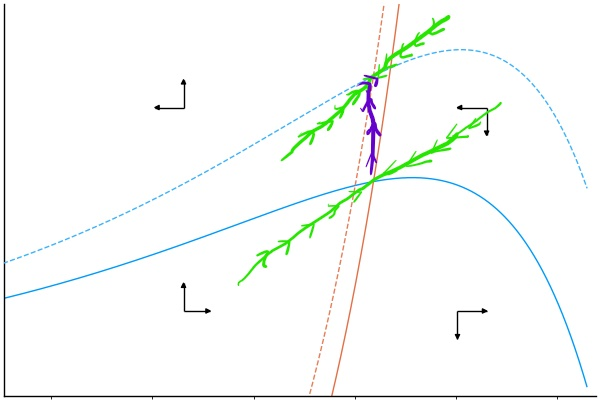
\includegraphics{fig1_LI.jpg}

    \hypertarget{continuing-from-4-compute-numerically-and-plot-trajectories-of-k_t-and-c_t-for-t12-ldots-20-if-the-productivity-shock-occurs-at-t_05-and-zprimez0.1-.-for-this-question-we-will-be-looking-at-the-linearized-version-of-the-nonlinear-system-around-the-new-steady-state.}{%
\subsection{\texorpdfstring{5. (continuing from 4) Compute numerically
and plot trajectories of \(k_{t}\) and \(c_{t}\) for
\(t=1,2, \ldots, 20\) if the productivity shock occurs at \(t_{0}=5\)
and \(z^{\prime}=z+0.1 .\) For this question, we will be looking at the
linearized version of the nonlinear system around the new steady
state.}{5. (continuing from 4) Compute numerically and plot trajectories of k\_\{t\} and c\_\{t\} for t=1,2, \textbackslash ldots, 20 if the productivity shock occurs at t\_\{0\}=5 and z\^{}\{\textbackslash prime\}=z+0.1 . For this question, we will be looking at the linearized version of the nonlinear system around the new steady state.}}\label{continuing-from-4-compute-numerically-and-plot-trajectories-of-k_t-and-c_t-for-t12-ldots-20-if-the-productivity-shock-occurs-at-t_05-and-zprimez0.1-.-for-this-question-we-will-be-looking-at-the-linearized-version-of-the-nonlinear-system-around-the-new-steady-state.}}

\hypertarget{a-compute-the-new-steady-state-leftbarkprime-barcprimeright-.-and-jacobian-matrix-at-that-point.}{%
\subsubsection{\texorpdfstring{(a) Compute the new steady state
\(\left(\bar{k}^{\prime}, \bar{c}^{\prime}\right) .\) and Jacobian
matrix at that
point.}{(a) Compute the new steady state \textbackslash left(\textbackslash bar\{k\}\^{}\{\textbackslash prime\}, \textbackslash bar\{c\}\^{}\{\textbackslash prime\}\textbackslash right) . and Jacobian matrix at that point.}}\label{a-compute-the-new-steady-state-leftbarkprime-barcprimeright-.-and-jacobian-matrix-at-that-point.}}

We will use the same formulas as before, but changing \(z\) from \(1\)
to \(1.1\).
\begin{Verbatim}[commandchars=\\\{\}]
{\color{incolor}In [{\color{incolor}31}]:} \PY{c}{\PYZpc{} new steady state}
         \PY{n}{z} \PY{p}{=} \PY{n}{z} \PY{o}{+} \PY{l+m+mf}{0.1}\PY{p}{;}
         \PY{n}{k\PYZus{}bar\PYZus{}2} \PY{p}{=} \PY{p}{(}\PY{l+m+mi}{1} \PY{o}{/}\PY{p}{(}\PY{n}{z} \PY{o}{*} \PY{n}{alpha}\PY{p}{)} \PY{o}{*} \PY{p}{(}\PY{l+m+mi}{1}\PY{o}{/}\PY{n+nb}{beta}\PY{o}{\PYZhy{}}\PY{p}{(}\PY{l+m+mi}{1}\PY{o}{\PYZhy{}}\PY{n}{delta}\PY{p}{)}\PY{p}{)}\PY{p}{)}\PYZca{}\PY{p}{(}\PY{l+m+mi}{1}\PY{o}{/}\PY{p}{(}\PY{n}{alpha}\PY{o}{\PYZhy{}}\PY{l+m+mi}{1}\PY{p}{)}\PY{p}{)}
         \PY{n}{c\PYZus{}bar\PYZus{}2} \PY{p}{=} \PY{n}{z}\PY{o}{*}\PY{n}{k\PYZus{}bar}\PYZca{}\PY{n}{alpha} \PY{o}{\PYZhy{}} \PY{n}{delta}\PY{o}{*}\PY{n}{k\PYZus{}bar}
\end{Verbatim}

    \begin{Verbatim}[commandchars=\\\{\}]
k\_bar\_2 =
    3.7458
c\_bar\_2 =
    1.2424


    \end{Verbatim}
\begin{Verbatim}[commandchars=\\\{\}]
{\color{incolor}In [{\color{incolor}32}]:} \PY{c}{\PYZpc{} Jacobian matrix at new steady state}
         \PY{n}{J2\PYZus{}11} \PY{p}{=}  \PY{n}{alpha}\PY{o}{*}\PY{n}{z}\PY{o}{*}\PY{n}{k\PYZus{}bar}\PYZca{}\PY{p}{(}\PY{n}{alpha} \PY{o}{\PYZhy{}}\PY{l+m+mi}{1}\PY{p}{)}\PY{o}{+}\PY{p}{(}\PY{l+m+mi}{1}\PY{o}{\PYZhy{}}\PY{n}{delta}\PY{p}{)} \PY{p}{;}
         \PY{n}{J2\PYZus{}12} \PY{p}{=}  \PY{o}{\PYZhy{}}\PY{l+m+mi}{1} \PY{p}{;}
         \PY{n}{J2\PYZus{}21} \PY{p}{=} \PY{p}{(}\PY{n}{alpha}\PY{o}{\PYZhy{}}\PY{l+m+mi}{1}\PY{p}{)}\PY{o}{*}\PY{n}{alpha}\PY{o}{*}\PY{n+nb}{beta}\PY{o}{*}\PY{n}{z}\PY{o}{*}\PY{n}{c\PYZus{}bar}\PY{o}{*}\PY{p}{(}\PY{n}{z}\PY{o}{*}\PY{n}{k\PYZus{}bar}\PYZca{}\PY{n}{alpha}\PY{o}{+}\PY{p}{(}\PY{l+m+mi}{1}\PY{o}{\PYZhy{}}\PY{n}{delta}\PY{p}{)}\PY{o}{*}\PY{n}{k\PYZus{}bar}\PY{o}{\PYZhy{}}\PY{n}{c\PYZus{}bar}\PY{p}{)}\PYZca{}\PY{p}{(}\PY{n}{alpha}\PY{o}{\PYZhy{}}\PY{l+m+mi}{2}\PY{p}{)}\PY{p}{;}
         \PY{n}{J2\PYZus{}22} \PY{p}{=}  \PY{n+nb}{beta}\PY{o}{*}\PY{p}{(}\PY{n}{alpha}\PY{o}{*}\PY{n}{z}\PY{o}{*}\PY{p}{(}\PY{o}{\PYZhy{}}\PY{n}{c\PYZus{}bar}\PY{o}{+}\PY{p}{(}\PY{l+m+mi}{1}\PY{o}{\PYZhy{}}\PY{n}{delta} \PY{p}{)}\PY{o}{*}\PY{n}{k\PYZus{}bar}\PY{o}{+}\PY{n}{z}\PY{o}{*}\PY{n}{k\PYZus{}bar}\PYZca{}\PY{n}{alpha}\PY{p}{)}\PYZca{}\PY{p}{(}\PY{n}{alpha}
         \PY{o}{\PYZhy{}}\PY{l+m+mi}{1}\PY{p}{)}\PY{o}{\PYZhy{}}\PY{n}{delta}\PY{o}{+}\PY{l+m+mi}{1}\PY{p}{)}\PY{o}{\PYZhy{}}\PY{p}{(}\PY{n}{alpha} \PY{o}{\PYZhy{}}\PY{l+m+mi}{1}\PY{p}{)}\PY{o}{*}\PY{n}{alpha}\PY{o}{*}\PY{n+nb}{beta}\PY{o}{*}\PY{n}{z}\PY{o}{*}\PY{n}{c\PYZus{}bar}\PY{o}{*}\PY{p}{(}\PY{o}{\PYZhy{}}\PY{n}{c\PYZus{}bar}\PY{o}{+}\PY{p}{(}\PY{l+m+mi}{1}\PY{o}{\PYZhy{}}\PY{n}{delta}\PY{p}{)}\PY{o}{*}\PY{n}{k\PYZus{}bar}\PY{o}{+}\PY{n}{z}\PY{o}{*}\PY{n}{k\PYZus{}bar}\PYZca{}\PY{n}{alpha}\PY{p}{)}\PYZca{}\PY{p}{(}\PY{n}{alpha}
         \PY{o}{\PYZhy{}}\PY{l+m+mi}{2}\PY{p}{)}\PY{p}{;}
         \PY{n}{J2} \PY{p}{=} \PY{p}{[}\PY{n}{J2\PYZus{}11}\PY{p}{,} \PY{n}{J2\PYZus{}12}\PY{p}{;} \PY{n}{J2\PYZus{}21}\PY{p}{,} \PY{n}{J2\PYZus{}22}\PY{p}{]}
\end{Verbatim}

    \begin{Verbatim}[commandchars=\\\{\}]
J2 =
    1.0440   -1.0000
   -0.0306    1.0392


    \end{Verbatim}

    \hypertarget{b-diagonalize-the-system-using-eigenvectors-and-rewrite-it-in-terms-of-hatk_t-and-hatc_t}{%
\subsubsection{\texorpdfstring{(b) Diagonalize the system using
eigenvectors and rewrite it in terms of \(\hat{k}_{t}\) and
\(\hat{c}_{t}:\)}{(b) Diagonalize the system using eigenvectors and rewrite it in terms of \textbackslash hat\{k\}\_\{t\} and \textbackslash hat\{c\}\_\{t\}:}}\label{b-diagonalize-the-system-using-eigenvectors-and-rewrite-it-in-terms-of-hatk_t-and-hatc_t}}

We know that \[
E^{-1} J E=\Lambda
\]

where \(E\) is the matrix of that have the eigenvectors of \(J\) as
columns and \(\Lambda\) is the diagonal matrix of eigenvectors.

Then:

    \[
\begin{array}{c}
E^{-1}\left(\begin{array}{c}
\tilde{k}_{t+1} \\
\tilde{c}_{t+1}
\end{array}\right)=\Lambda E^{-1}\left(\begin{array}{c}
\tilde{k}_{t} \\
\tilde{c}_{t}
\end{array}\right) \\
\left(\begin{array}{c}
\hat{k}_{t+1} \\
\hat{c}_{t+1}
\end{array}\right)=\Lambda\left(\begin{array}{c}
\hat{k}_{t} \\
\hat{c}_{t}
\end{array}\right)
\end{array}
\]

    We can define then the system as:

\[
\left(\begin{array}{l}
\hat{k}_{t+1} \\
\hat{c}_{t+1}
\end{array}\right)=\Lambda\left(\begin{array}{l}
\hat{k}_{t} \\
\hat{c}_{t}
\end{array}\right)
\]

To find the numerical values we do:
\begin{Verbatim}[commandchars=\\\{\}]
{\color{incolor}In [{\color{incolor}33}]:} \PY{c}{\PYZpc{} eigenvalues and eigenvectors}
         \PY{p}{[}\PY{n}{V2}\PY{p}{,}\PY{n}{D2}\PY{p}{]}\PY{p}{=}\PY{n}{eig}\PY{p}{(}\PY{n}{J2}\PY{p}{)}
\end{Verbatim}

    \begin{Verbatim}[commandchars=\\\{\}]
V2 =
    0.9854    0.9846
   -0.1700    0.1746
D2 =
    1.2165         0
         0    0.8667


    \end{Verbatim}

    \hypertarget{c-write-down-non-explosive-solution-for-lefthatk_t-hatc_tright-rewrite-in-terms-of-original-variables-leftk_t-c_tright}{%
\subsubsection{\texorpdfstring{(c) Write down non-explosive solution for
\(\left(\hat{k}_{t}, \hat{c}_{t}\right),\) rewrite in terms of original
variables
\(\left(k_{t}, c_{t}\right)\)}{(c) Write down non-explosive solution for \textbackslash left(\textbackslash hat\{k\}\_\{t\}, \textbackslash hat\{c\}\_\{t\}\textbackslash right), rewrite in terms of original variables \textbackslash left(k\_\{t\}, c\_\{t\}\textbackslash right)}}\label{c-write-down-non-explosive-solution-for-lefthatk_t-hatc_tright-rewrite-in-terms-of-original-variables-leftk_t-c_tright}}

Since \(\lambda_1>1\) the non explosive solution is only in terms of
\(\lambda_{2}\), this is: \[\hat{k}_t = 0\]
\[\hat{c}_t = c \lambda_2^t\]

We can recover the solution in the original variables by \[
\begin{array}{c}
\left(\begin{array}{c}
k_{1}-\bar{k}^{\prime} \\
c_{t}-\bar{c}^{\prime}
\end{array}\right)=E\left(\begin{array}{c}
\hat{k}_{t} \\
\hat{c}_{t}
\end{array}\right)=\left(\begin{array}{c}
e_{11} \hat{k}_{t}+e_{12} \hat{c}_{t} \\
e_{21} \hat{k}_{t}+e_{22} \hat{c}_{t}
\end{array}\right) \\
\left(\begin{array}{c}
k_{t} \\
c_{t}
\end{array}\right)=\left(\begin{array}{c}
\bar{k}^{\prime}+e_{12} c_{2} \lambda_{2}^{t} \\
\bar{c}^{\prime}+e_{22} c_{2} \lambda_{2}^{t}
\end{array}\right)
\end{array}
\]

    \hypertarget{d-pin-down-a-particular-saddle-path-trajectory-using-a-boundary-condition-k_t_0bark-capital-cant-jump-from-the-old-steady-state-at-the-time-of-the-shock-so-pick-suitable-c_t_0-.}{%
\subsubsection{\texorpdfstring{(d) Pin down a particular saddle path
trajectory using a boundary condition \(k_{t_{0}}=\bar{k}\) (capital
can't jump from the old steady state at the time of the shock, so pick
suitable \(c_{t_{0}}\)
).}{(d) Pin down a particular saddle path trajectory using a boundary condition k\_\{t\_\{0\}\}=\textbackslash bar\{k\} (capital can't jump from the old steady state at the time of the shock, so pick suitable c\_\{t\_\{0\}\} ).}}\label{d-pin-down-a-particular-saddle-path-trajectory-using-a-boundary-condition-k_t_0bark-capital-cant-jump-from-the-old-steady-state-at-the-time-of-the-shock-so-pick-suitable-c_t_0-.}}

We need the solution to start in the old steady state, this is: \[
k_{t_{0}}=\bar{k} = \bar{k}^{\prime}+e_{12} c \lambda_{2}^{t_0} 
\]
\begin{Verbatim}[commandchars=\\\{\}]
{\color{incolor}In [{\color{incolor}34}]:} \PY{n}{t0} \PY{p}{=} \PY{l+m+mi}{5}
         \PY{n}{syms} \PY{l+s}{c}
         \PY{n}{eqn} \PY{p}{=} \PY{n}{k\PYZus{}bar\PYZus{}2} \PY{o}{+} \PY{n}{V2}\PY{p}{(}\PY{l+m+mi}{1}\PY{p}{,}\PY{l+m+mi}{2}\PY{p}{)}\PY{o}{*}\PY{n}{c}\PY{o}{*}\PY{n}{D}\PY{p}{(}\PY{l+m+mi}{2}\PY{p}{,}\PY{l+m+mi}{2}\PY{p}{)}\PYZca{}\PY{n}{t0} \PY{o}{==} \PY{n}{k\PYZus{}bar}\PY{p}{;}
         
         \PY{n}{const} \PY{p}{=} \PY{n}{vpasolve}\PY{p}{(}\PY{n}{eqn}\PY{p}{,} \PY{n}{c}\PY{p}{)}
\end{Verbatim}

    \begin{Verbatim}[commandchars=\\\{\}]
t0 =
     5
const =
-1.0446432524311788851461547566629


    \end{Verbatim}
\begin{Verbatim}[commandchars=\\\{\}]
{\color{incolor}In [{\color{incolor}35}]:} \PY{p}{(}\PY{n}{k\PYZus{}bar} \PY{o}{\PYZhy{}} \PY{n}{k\PYZus{}bar\PYZus{}2}\PY{p}{)}\PY{o}{/}\PY{p}{(}\PY{n}{V2}\PY{p}{(}\PY{l+m+mi}{1}\PY{p}{,}\PY{l+m+mi}{2}\PY{p}{)}\PY{o}{*}\PY{n}{D}\PY{p}{(}\PY{l+m+mi}{2}\PY{p}{,}\PY{l+m+mi}{2}\PY{p}{)}\PYZca{}\PY{n}{t0}\PY{p}{)}
\end{Verbatim}

    \begin{Verbatim}[commandchars=\\\{\}]
ans =
   -1.0446


    \end{Verbatim}

    \hypertarget{e-use-the-particular-solution-to-compute-and-graph-k_t-and-c_t-after-the-shock.}{%
\subsubsection{\texorpdfstring{(e) Use the particular solution to
compute and graph \(k_{t}\) and \(c_{t}\) after the
shock.}{(e) Use the particular solution to compute and graph k\_\{t\} and c\_\{t\} after the shock.}}\label{e-use-the-particular-solution-to-compute-and-graph-k_t-and-c_t-after-the-shock.}}

With the value stored in the variable \(c =\)\texttt{const} we can
compute the particular solution:

\[
\begin{array}{c}
k_t = \bar{k}^{\prime}+e_{12} c \lambda_{2}^{t} \\
c_t = \bar{c}^{\prime}+e_{22} c \lambda_{2}^{t}
\end{array}
\]
\begin{Verbatim}[commandchars=\\\{\}]
{\color{incolor}In [{\color{incolor}36}]:} \PY{n}{t} \PY{p}{=} \PY{l+m+mi}{0}\PY{p}{:}\PY{l+m+mi}{20}\PY{p}{;}
         \PY{n}{k\PYZus{}t} \PY{p}{=} \PY{n}{k\PYZus{}bar\PYZus{}2}\PY{o}{+}\PY{n}{V2}\PY{p}{(}\PY{l+m+mi}{1}\PY{p}{,}\PY{l+m+mi}{2}\PY{p}{)}\PY{o}{*}\PY{n}{const}\PY{o}{*}\PY{n}{D}\PY{p}{(}\PY{l+m+mi}{2}\PY{p}{,}\PY{l+m+mi}{2}\PY{p}{)}\PY{o}{.\PYZca{}}\PY{n}{t}\PY{p}{;}
         \PY{n}{c\PYZus{}t} \PY{p}{=} \PY{n}{c\PYZus{}bar\PYZus{}2}\PY{o}{+}\PY{n}{V2}\PY{p}{(}\PY{l+m+mi}{2}\PY{p}{,}\PY{l+m+mi}{2}\PY{p}{)}\PY{o}{*}\PY{n}{const}\PY{o}{*}\PY{n}{D}\PY{p}{(}\PY{l+m+mi}{2}\PY{p}{,}\PY{l+m+mi}{2}\PY{p}{)}\PY{o}{.\PYZca{}}\PY{n}{t}\PY{p}{;}
         \PY{n}{figure}
         \PY{l+s}{hold} \PY{l+s}{on}
         \PY{n}{subplot}\PY{p}{(}\PY{l+m+mi}{2}\PY{p}{,}\PY{l+m+mi}{1}\PY{p}{,}\PY{l+m+mi}{1}\PY{p}{)}
         \PY{n}{plot}\PY{p}{(}\PY{l+m+mi}{1}\PY{p}{:}\PY{l+m+mi}{20}\PY{p}{,} \PY{p}{[}\PY{n+nb}{repmat}\PY{p}{(}\PY{n}{k\PYZus{}bar}\PY{p}{,} \PY{l+m+mi}{1}\PY{p}{,}\PY{l+m+mi}{4}\PY{p}{)}\PY{p}{,} \PY{n}{k\PYZus{}t}\PY{p}{(}\PY{l+m+mi}{6}\PY{p}{:}\PY{k}{end}\PY{p}{)}\PY{p}{]}\PY{p}{,} \PY{l+s}{\PYZdq{}\PYZhy{}*\PYZdq{}}\PY{p}{)}
         \PY{n}{h} \PY{p}{=} \PY{n}{title}\PY{p}{(}\PY{l+s}{\PYZsq{}}\PY{l+s}{\PYZdl{}k\PYZus{}t\PYZdl{}\PYZsq{}}\PY{p}{,} \PY{l+s}{\PYZsq{}}\PY{l+s}{interpreter\PYZsq{}}\PY{p}{,} \PY{l+s}{\PYZsq{}}\PY{l+s}{latex\PYZsq{}}\PY{p}{)}\PY{p}{;}
         \PY{n}{h}\PY{p}{.}\PY{n}{FontSize}\PY{p}{=}\PY{l+m+mi}{15}\PY{p}{;}
         \PY{n}{subplot}\PY{p}{(}\PY{l+m+mi}{2}\PY{p}{,}\PY{l+m+mi}{1}\PY{p}{,}\PY{l+m+mi}{2}\PY{p}{)}
         \PY{n}{plot}\PY{p}{(}\PY{l+m+mi}{1}\PY{p}{:}\PY{l+m+mi}{20}\PY{p}{,} \PY{p}{[}\PY{n+nb}{repmat}\PY{p}{(}\PY{n}{c\PYZus{}bar}\PY{p}{,} \PY{l+m+mi}{1}\PY{p}{,}\PY{l+m+mi}{4}\PY{p}{)}\PY{p}{,} \PY{n}{c\PYZus{}t}\PY{p}{(}\PY{l+m+mi}{6}\PY{p}{:}\PY{k}{end}\PY{p}{)}\PY{p}{]}\PY{p}{,} \PY{l+s}{\PYZdq{}\PYZhy{}*\PYZdq{}}\PY{p}{)}
         \PY{n}{h} \PY{p}{=} \PY{n}{xlabel}\PY{p}{(}\PY{l+s}{\PYZsq{}}\PY{l+s}{Time\PYZsq{}}\PY{p}{,} \PY{l+s}{\PYZsq{}}\PY{l+s}{interpreter\PYZsq{}}\PY{p}{,} \PY{l+s}{\PYZsq{}}\PY{l+s}{latex\PYZsq{}}\PY{p}{)}\PY{p}{;}
         \PY{n}{h}\PY{p}{.}\PY{n}{FontSize}\PY{p}{=}\PY{l+m+mi}{13}\PY{p}{;}
         \PY{n}{h} \PY{p}{=} \PY{n}{title}\PY{p}{(}\PY{l+s}{\PYZsq{}}\PY{l+s}{\PYZdl{}c\PYZus{}t\PYZdl{}\PYZsq{}}\PY{p}{,} \PY{l+s}{\PYZsq{}}\PY{l+s}{interpreter\PYZsq{}}\PY{p}{,} \PY{l+s}{\PYZsq{}}\PY{l+s}{latex\PYZsq{}}\PY{p}{)}\PY{p}{;}
         \PY{n}{h}\PY{p}{.}\PY{n}{FontSize}\PY{p}{=}\PY{l+m+mi}{15}\PY{p}{;}
         
         \PY{n}{set}\PY{p}{(}\PY{n}{gca}\PY{p}{,}\PY{l+s}{\PYZsq{}}\PY{l+s}{TickLabelInterpreter\PYZsq{}}\PY{p}{,}\PY{l+s}{\PYZsq{}}\PY{l+s}{latex\PYZsq{}}\PY{p}{)}
\end{Verbatim}

    \begin{Verbatim}[commandchars=\\\{\}]


    \end{Verbatim}

    \begin{center}
    \adjustimage{max size={0.9\linewidth}{0.9\paperheight}}{Problem_Set_2_files/Problem_Set_2_30_1.png}
    \end{center}
    { \hspace*{\fill} \\}
    
    \hypertarget{for-this-question-we-explore-the-nonlinear-nature-of-the-system-and-numerically-solve-the-actual-transition-path-using-the-shooting-method.}{%
\subsection{6. For this question, we explore the nonlinear nature of the
system and numerically solve the actual transition path using the
``shooting
method''.}\label{for-this-question-we-explore-the-nonlinear-nature-of-the-system-and-numerically-solve-the-actual-transition-path-using-the-shooting-method.}}

\hypertarget{a-in-the-previous-question-you-solve-c_t_0-under-the-linear-system.-put-leftk_t_0-c_t_0right-into-the-nonlinear-system-1a-and-1b.-compute-and-graph-how-the-system-evolves.-does-it-converge-to-a-steady-state}{%
\subsubsection{\texorpdfstring{(a) In the previous question, you solve
\(c_{t_{0}}\) under the linear system. Put
\(\left(k_{t_{0}}, c_{t_{0}}\right)\) into the nonlinear system \((1a)\)
and \((1b)\). Compute and graph how the system evolves. Does it converge
to a steady
state?}{(a) In the previous question, you solve c\_\{t\_\{0\}\} under the linear system. Put \textbackslash left(k\_\{t\_\{0\}\}, c\_\{t\_\{0\}\}\textbackslash right) into the nonlinear system (1a) and (1b). Compute and graph how the system evolves. Does it converge to a steady state?}}\label{a-in-the-previous-question-you-solve-c_t_0-under-the-linear-system.-put-leftk_t_0-c_t_0right-into-the-nonlinear-system-1a-and-1b.-compute-and-graph-how-the-system-evolves.-does-it-converge-to-a-steady-state}}
\begin{Verbatim}[commandchars=\\\{\}]
{\color{incolor}In [{\color{incolor}38}]:} \PY{n}{c\PYZus{}t0} \PY{p}{=} \PY{n}{c\PYZus{}bar\PYZus{}2} \PY{o}{+} \PY{n}{V2}\PY{p}{(}\PY{l+m+mi}{2}\PY{p}{,}\PY{l+m+mi}{2}\PY{p}{)}\PY{o}{*}\PY{n}{const}\PY{o}{*}\PY{p}{(}\PY{n}{D2}\PY{p}{(}\PY{l+m+mi}{2}\PY{p}{,}\PY{l+m+mi}{2}\PY{p}{)}\PY{o}{.\PYZca{}}\PY{n}{t0}\PY{p}{)}
\end{Verbatim}

    \begin{Verbatim}[commandchars=\\\{\}]
c\_t0 =
1.1532439993949588711552818657191


    \end{Verbatim}
\begin{Verbatim}[commandchars=\\\{\}]
{\color{incolor}In [{\color{incolor}39}]:} \PY{n}{Prd} \PY{p}{=} \PY{l+m+mi}{20}\PY{o}{\PYZhy{}}\PY{n}{t0}\PY{o}{+}\PY{l+m+mi}{1}\PY{p}{;}
         
         \PY{n}{Trj1} \PY{p}{=} \PY{n+nb}{zeros}\PY{p}{(}\PY{l+m+mi}{2}\PY{p}{,}\PY{n}{Prd}\PY{p}{)}\PY{p}{;}
         \PY{n}{Trj1}\PY{p}{(}\PY{l+m+mi}{1}\PY{p}{,}\PY{l+m+mi}{1}\PY{p}{)} \PY{p}{=} \PY{n}{k\PYZus{}bar}\PY{p}{;}   \PY{c}{\PYZpc{} At t0, agent are stuck with k\PYZus{}bar}
         \PY{n}{Trj1}\PY{p}{(}\PY{l+m+mi}{2}\PY{p}{,}\PY{l+m+mi}{1}\PY{p}{)} \PY{p}{=} \PY{n}{c\PYZus{}t0}\PY{p}{;}     \PY{c}{\PYZpc{} They can choose consumption so that they will fall onto the new}
         \PY{n}{saddle} \PY{l+s}{path}
         \PY{k}{for} \PY{n+nb}{i} \PY{p}{=} \PY{l+m+mi}{2}\PY{p}{:}\PY{n}{Prd}
             \PY{n}{Trj1}\PY{p}{(}\PY{p}{:}\PY{p}{,}\PY{n+nb}{i}\PY{p}{)}\PY{p}{=} \PY{n}{J}\PY{o}{*}\PY{n}{Trj1}\PY{p}{(}\PY{p}{:}\PY{p}{,}\PY{n+nb}{i}\PY{o}{\PYZhy{}}\PY{l+m+mi}{1}\PY{p}{)}\PY{p}{;} \PY{c}{\PYZpc{} Fill in the system dynamics, i.e. relating Trj1(:,i) to}
         \PY{n}{Trj1}\PY{p}{(}\PY{p}{:}\PY{p}{,}\PY{n+nb}{i}\PY{o}{\PYZhy{}}\PY{l+m+mi}{1}\PY{p}{)} \PY{n}{using} \PY{l+m+mi}{2}\PY{p}{(}\PY{n}{c}\PY{p}{)}\PY{p}{;}
         \PY{n}{end}
\end{Verbatim}

    \begin{Verbatim}[commandchars=\\\{\}]


    \end{Verbatim}
\begin{Verbatim}[commandchars=\\\{\}]
{\color{incolor}In [{\color{incolor}40}]:} \PY{n}{Trj2} \PY{p}{=} \PY{n+nb}{zeros}\PY{p}{(}\PY{l+m+mi}{2}\PY{p}{,}\PY{n}{Prd}\PY{p}{)}\PY{p}{;}
         \PY{n}{Trj2}\PY{p}{(}\PY{l+m+mi}{1}\PY{p}{,}\PY{l+m+mi}{1}\PY{p}{)}\PY{p}{=}\PY{n}{k\PYZus{}bar}\PY{p}{;}
         \PY{n}{Trj2}\PY{p}{(}\PY{l+m+mi}{2}\PY{p}{,}\PY{l+m+mi}{1}\PY{p}{)}\PY{p}{=}\PY{n}{c\PYZus{}t0}\PY{p}{;}
         \PY{n}{for} \PY{l+s}{i} \PY{l+s}{=} \PY{l+s}{2:Prd}
             \PY{n}{k} \PY{p}{=} \PY{n}{Trj2}\PY{p}{(}\PY{l+m+mi}{1}\PY{p}{,}\PY{n+nb}{i}\PY{o}{\PYZhy{}}\PY{l+m+mi}{1}\PY{p}{)}\PY{p}{;}
             \PY{n}{c} \PY{p}{=} \PY{n}{Trj2}\PY{p}{(}\PY{l+m+mi}{2}\PY{p}{,}\PY{n+nb}{i}\PY{o}{\PYZhy{}}\PY{l+m+mi}{1}\PY{p}{)}\PY{p}{;}
             \PY{n}{Trj2}\PY{p}{(}\PY{l+m+mi}{1}\PY{p}{,}\PY{n+nb}{i}\PY{p}{)} \PY{p}{=} \PY{n}{z}\PY{o}{*}\PY{n}{k}\PY{o}{.\PYZca{}}\PY{n}{alpha} \PY{o}{+} \PY{p}{(}\PY{l+m+mi}{1}\PY{o}{\PYZhy{}}\PY{n}{delta}\PY{p}{)}\PY{o}{*}\PY{n}{k} \PY{o}{\PYZhy{}} \PY{n}{c}\PY{p}{;}
             \PY{n}{Trj2}\PY{p}{(}\PY{l+m+mi}{2}\PY{p}{,}\PY{n+nb}{i}\PY{p}{)} \PY{p}{=} \PY{p}{(}\PY{l+m+mi}{1}\PY{o}{\PYZhy{}}\PY{n}{delta}\PY{o}{+}\PY{n}{z}\PY{o}{*}\PY{n}{alpha}\PY{o}{*}\PY{n}{k}\PY{o}{.\PYZca{}}\PY{p}{(}\PY{n}{alpha}\PY{o}{\PYZhy{}}\PY{l+m+mi}{1}\PY{p}{)}\PY{p}{)}\PY{o}{*}\PY{n+nb}{beta}\PY{o}{*}\PY{n}{c}\PY{p}{;}
         \PY{n}{end}
\end{Verbatim}

    \begin{Verbatim}[commandchars=\\\{\}]


    \end{Verbatim}
\begin{Verbatim}[commandchars=\\\{\}]
{\color{incolor}In [{\color{incolor}41}]:} \PY{n}{before} \PY{p}{=} \PY{n+nb}{repmat}\PY{p}{(}\PY{p}{[}\PY{n}{k\PYZus{}bar}\PY{p}{;} \PY{n}{c\PYZus{}bar}\PY{p}{]}\PY{p}{,}\PY{l+m+mi}{1}\PY{p}{,} \PY{n}{t0}\PY{o}{\PYZhy{}}\PY{l+m+mi}{1}\PY{p}{)}\PY{p}{;}
         \PY{n}{Trj1\PYZus{}whole} \PY{p}{=} \PY{p}{[}\PY{n}{before}\PY{p}{,} \PY{n}{Trj1}\PY{p}{]}\PY{p}{;}   \PY{c}{\PYZpc{} Transition under linear hypothesis}
         \PY{n}{Trj2\PYZus{}whole} \PY{p}{=} \PY{p}{[}\PY{n}{before}\PY{p}{,} \PY{n}{Trj2}\PY{p}{]}\PY{p}{;}   \PY{c}{\PYZpc{} Actual transition using \PYZdq{}jump\PYZdq{} from linearization}
\end{Verbatim}

    \begin{Verbatim}[commandchars=\\\{\}]


    \end{Verbatim}
\begin{Verbatim}[commandchars=\\\{\}]
{\color{incolor}In [{\color{incolor}42}]:} \PY{n}{time} \PY{p}{=} \PY{l+m+mi}{1}\PY{p}{:}\PY{l+m+mi}{20}\PY{p}{;}
         \PY{n}{figure}
         \PY{l+s}{subplot(2,1,1)}       \PY{l+s}{\PYZpc{}} \PY{l+s}{add} \PY{l+s}{first} \PY{l+s}{plot} \PY{l+s}{in} \PY{l+s}{2} \PY{l+s}{x} \PY{l+s}{1} \PY{l+s}{grid}
         \PY{n}{plot}\PY{p}{(}\PY{n}{time}\PY{p}{,}\PY{n}{Trj2\PYZus{}whole}\PY{p}{(}\PY{l+m+mi}{1}\PY{p}{,}\PY{p}{:}\PY{p}{)}\PY{p}{,}\PY{l+s}{\PYZsq{}}\PY{l+s}{\PYZhy{}*\PYZsq{}}\PY{p}{)}
         \PY{n}{title}\PY{p}{(}\PY{l+s}{\PYZsq{}}\PY{l+s}{\PYZdl{}k\PYZus{}t\PYZdl{}\PYZsq{}}\PY{p}{,} \PY{l+s}{\PYZsq{}}\PY{l+s}{interpreter\PYZsq{}}\PY{p}{,} \PY{l+s}{\PYZsq{}}\PY{l+s}{latex\PYZsq{}}\PY{p}{)}\PY{p}{;}
         \PY{n}{subplot}\PY{p}{(}\PY{l+m+mi}{2}\PY{p}{,}\PY{l+m+mi}{1}\PY{p}{,}\PY{l+m+mi}{2}\PY{p}{)}       \PY{c}{\PYZpc{} add first plot in 2 x 1 grid}
         \PY{n}{plot}\PY{p}{(}\PY{n}{time}\PY{p}{,}\PY{n}{Trj2\PYZus{}whole}\PY{p}{(}\PY{l+m+mi}{2}\PY{p}{,}\PY{p}{:}\PY{p}{)}\PY{p}{,}\PY{l+s}{\PYZsq{}}\PY{l+s}{\PYZhy{}*\PYZsq{}}\PY{p}{)}
         \PY{n}{xlabel}\PY{p}{(}\PY{l+s}{\PYZsq{}}\PY{l+s}{Time\PYZsq{}}\PY{p}{,} \PY{l+s}{\PYZsq{}}\PY{l+s}{interpreter\PYZsq{}}\PY{p}{,} \PY{l+s}{\PYZsq{}}\PY{l+s}{latex\PYZsq{}}\PY{p}{)}\PY{p}{;}
         \PY{n}{title}\PY{p}{(}\PY{l+s}{\PYZsq{}}\PY{l+s}{\PYZdl{}c\PYZus{}t\PYZdl{}\PYZsq{}}\PY{p}{,} \PY{l+s}{\PYZsq{}}\PY{l+s}{interpreter\PYZsq{}}\PY{p}{,} \PY{l+s}{\PYZsq{}}\PY{l+s}{latex\PYZsq{}}\PY{p}{)}\PY{p}{;}
         \PY{n}{set}\PY{p}{(}\PY{n}{gca}\PY{p}{,}\PY{l+s}{\PYZsq{}}\PY{l+s}{TickLabelInterpreter\PYZsq{}}\PY{p}{,}\PY{l+s}{\PYZsq{}}\PY{l+s}{latex\PYZsq{}}\PY{p}{)}
\end{Verbatim}

    \begin{Verbatim}[commandchars=\\\{\}]


    \end{Verbatim}

    \begin{center}
    \adjustimage{max size={0.9\linewidth}{0.9\paperheight}}{Problem_Set_2_files/Problem_Set_2_36_1.png}
    \end{center}
    { \hspace*{\fill} \\}
    
    We can observe in the figure above that the system does not converges to
the steady state.

    \hypertarget{b-use-shooting-method-to-find-the-actual-c_t_0-needed.-the-method-is-to-try-different-values-of-c_t_0-such-that-after-long-enough-time-the-system-will-converge-to-the-new-steady-state.}{%
\subsubsection{\texorpdfstring{(b) Use ``shooting method'' to find the
actual \(c_{t_{0}}\) needed. The method is to try different values of
\(c_{t_{0}}\) such that after long enough time, the system will converge
to the new steady
state.}{(b) Use ``shooting method'' to find the actual c\_\{t\_\{0\}\} needed. The method is to try different values of c\_\{t\_\{0\}\} such that after long enough time, the system will converge to the new steady state.}}\label{b-use-shooting-method-to-find-the-actual-c_t_0-needed.-the-method-is-to-try-different-values-of-c_t_0-such-that-after-long-enough-time-the-system-will-converge-to-the-new-steady-state.}}
\begin{Verbatim}[commandchars=\\\{\}]
{\color{incolor}In [{\color{incolor}189}]:} \PY{c}{\PYZpc{}\PYZpc{}file Utils/calib.m}
          \PY{k}{function}\PY{+w}{ }[ D ] \PY{p}{=}\PY{+w}{ }\PY{n+nf}{calib}\PY{p}{(} c\PYZus{}in, alpha, beta, delta, z, k\PYZus{}bar, k\PYZus{}bar2, c\PYZus{}bar2\PY{p}{)}
          \PY{c}{\PYZpc{} this function gives the distance to the new steady state after 30}
          \PY{c}{\PYZpc{} periods given the initial capital k\PYZus{}bar and consumption c\PYZus{}star}
          \PY{n}{T} \PY{p}{=} \PY{l+m+mi}{50}\PY{p}{;}
          \PY{n}{Trj} \PY{p}{=} \PY{n+nb}{zeros}\PY{p}{(}\PY{l+m+mi}{2}\PY{p}{,}\PY{n}{T}\PY{p}{)}\PY{p}{;}
          \PY{n}{Trj}\PY{p}{(}\PY{l+m+mi}{1}\PY{p}{,}\PY{l+m+mi}{1}\PY{p}{)} \PY{p}{=} \PY{n}{k\PYZus{}bar}\PY{p}{;}
          \PY{n}{Trj}\PY{p}{(}\PY{l+m+mi}{2}\PY{p}{,}\PY{l+m+mi}{1}\PY{p}{)} \PY{p}{=} \PY{n}{c\PYZus{}in}\PY{p}{;}
          \PY{n}{for} \PY{l+s}{i} \PY{l+s}{=} \PY{l+s}{2:T}
              \PY{n}{k} \PY{p}{=} \PY{n}{Trj}\PY{p}{(}\PY{l+m+mi}{1}\PY{p}{,}\PY{n+nb}{i}\PY{o}{\PYZhy{}}\PY{l+m+mi}{1}\PY{p}{)}\PY{p}{;}
              \PY{n}{c} \PY{p}{=} \PY{n}{Trj}\PY{p}{(}\PY{l+m+mi}{2}\PY{p}{,}\PY{n+nb}{i}\PY{o}{\PYZhy{}}\PY{l+m+mi}{1}\PY{p}{)}\PY{p}{;}
              \PY{n}{Trj}\PY{p}{(}\PY{l+m+mi}{1}\PY{p}{,}\PY{n+nb}{i}\PY{p}{)} \PY{p}{=} \PY{n}{z}\PY{o}{*}\PY{n}{k}\PY{o}{.\PYZca{}}\PY{n}{alpha} \PY{o}{+} \PY{p}{(}\PY{l+m+mi}{1}\PY{o}{\PYZhy{}}\PY{n}{delta}\PY{p}{)}\PY{o}{*}\PY{n}{k} \PY{o}{\PYZhy{}} \PY{n}{c}\PY{p}{;}
              \PY{n}{Trj}\PY{p}{(}\PY{l+m+mi}{2}\PY{p}{,}\PY{n+nb}{i}\PY{p}{)} \PY{p}{=} \PY{p}{(}\PY{l+m+mi}{1}\PY{o}{\PYZhy{}}\PY{n}{delta}\PY{o}{+}\PY{n}{z}\PY{o}{*}\PY{n}{alpha}\PY{o}{*}\PY{n}{k}\PY{o}{.\PYZca{}}\PY{p}{(}\PY{n}{alpha}\PY{o}{\PYZhy{}}\PY{l+m+mi}{1}\PY{p}{)}\PY{p}{)}\PY{o}{*}\PY{n+nb}{beta}\PY{o}{*}\PY{n}{c}\PY{p}{;}
          \PY{n}{end}
          \PY{l+s}{D} \PY{l+s}{=} \PY{l+s}{norm(Trj(:,T)\PYZhy{}[k\PYZus{}bar2}\PY{p}{;} \PY{n}{c\PYZus{}bar2}\PY{p}{]}\PY{p}{)}\PY{p}{;}
          \PY{c}{\PYZpc{} The norm function calculates the length of a vector}
\end{Verbatim}

    \begin{Verbatim}[commandchars=\\\{\}]
Created file 'P:\textbackslash{}PHD\textbackslash{}Courses\textbackslash{}ECON 712 Macro\textbackslash{}Notebooks (Mathematica Jupyter
Sage)\textbackslash{}Utils\textbackslash{}calib.m'.

    \end{Verbatim}
\begin{Verbatim}[commandchars=\\\{\}]
{\color{incolor}In [{\color{incolor}57}]:} \PY{n}{M} \PY{p}{=} \PY{l+m+mi}{10000}\PY{p}{;}  \PY{c}{\PYZpc{} Picking M number of candidates from c\PYZus{}t0}
         \PY{n}{C\PYZus{}range} \PY{p}{=} \PY{n+nb}{linspace}\PY{p}{(}\PY{n}{c\PYZus{}bar}\PY{p}{,} \PY{n}{c\PYZus{}bar\PYZus{}2}\PY{p}{,} \PY{n}{M}\PY{p}{)}\PY{p}{;}  \PY{c}{\PYZpc{} Choosing candidates of c\PYZus{}t0}
         \PY{n}{Distance} \PY{p}{=} \PY{n+nb}{zeros}\PY{p}{(}\PY{l+m+mi}{1}\PY{p}{,}\PY{n}{M}\PY{p}{)}\PY{p}{;}  \PY{c}{\PYZpc{} The matrix that stores the distance between the new steady}
         \PY{n}{state}
         \PY{l+s}{\PYZpc{}} \PY{l+s}{and} \PY{l+s}{where} \PY{l+s}{the} \PY{l+s}{system} \PY{l+s}{is} \PY{l+s}{at} \PY{l+s}{after} \PY{l+s}{a} \PY{l+s}{long} \PY{l+s}{period} \PY{l+s}{of} \PY{l+s}{time} \PY{l+s}{following}
         \PY{c}{\PYZpc{} particular c\PYZus{}t0}
         \PY{k}{for} \PY{n+nb}{i} \PY{p}{=} \PY{l+m+mi}{1}\PY{p}{:}\PY{n}{M}
             \PY{n}{Distance}\PY{p}{(}\PY{l+m+mi}{1}\PY{p}{,}\PY{n+nb}{i}\PY{p}{)}\PY{p}{=}\PY{n}{calib}\PY{p}{(} \PY{n}{c\PYZus{}t0}\PY{p}{,} \PY{n}{alpha}\PY{p}{,} \PY{n+nb}{beta}\PY{p}{,} \PY{n}{delta}\PY{p}{,} \PY{n}{z}\PY{p}{,} \PY{n}{k\PYZus{}bar}\PY{p}{,} \PY{n}{k\PYZus{}bar\PYZus{}2}\PY{p}{,} \PY{n}{c\PYZus{}bar\PYZus{}2}\PY{p}{)}\PY{p}{;}
         \PY{n}{end}
         \PY{l+s}{[DD,I]} \PY{l+s}{=} \PY{l+s}{min(Distance)}\PY{p}{;}     \PY{c}{\PYZpc{} Picking the particular c\PYZus{}t0 that minimizes the distance}
         \PY{n}{c\PYZus{}star} \PY{p}{=} \PY{n}{C\PYZus{}range}\PY{p}{(}\PY{n}{I}\PY{p}{)}\PY{p}{;}
\end{Verbatim}

    \begin{Verbatim}[commandchars=\\\{\}]


    \end{Verbatim}
\begin{Verbatim}[commandchars=\\\{\}]
{\color{incolor}In [{\color{incolor}58}]:} \PY{c}{\PYZpc{} Calibrating the actual nonlinear transition using c\PYZus{}star chosen above.}
         \PY{n}{Trj3} \PY{p}{=} \PY{n+nb}{zeros}\PY{p}{(}\PY{l+m+mi}{2}\PY{p}{,}\PY{n}{Prd}\PY{p}{)}\PY{p}{;}
         \PY{n}{Trj3}\PY{p}{(}\PY{l+m+mi}{1}\PY{p}{,}\PY{l+m+mi}{1}\PY{p}{)}\PY{p}{=}\PY{n}{k\PYZus{}bar}\PY{p}{;}
         \PY{n}{Trj3}\PY{p}{(}\PY{l+m+mi}{2}\PY{p}{,}\PY{l+m+mi}{1}\PY{p}{)}\PY{p}{=}\PY{n}{c\PYZus{}star}\PY{p}{;}
         \PY{n}{for} \PY{l+s}{i} \PY{l+s}{=} \PY{l+s}{2:Prd}
             \PY{n}{k} \PY{p}{=} \PY{n}{Trj3}\PY{p}{(}\PY{l+m+mi}{1}\PY{p}{,}\PY{n+nb}{i}\PY{o}{\PYZhy{}}\PY{l+m+mi}{1}\PY{p}{)}\PY{p}{;}
             \PY{n}{c} \PY{p}{=} \PY{n}{Trj3}\PY{p}{(}\PY{l+m+mi}{2}\PY{p}{,}\PY{n+nb}{i}\PY{o}{\PYZhy{}}\PY{l+m+mi}{1}\PY{p}{)}\PY{p}{;}
             \PY{n}{Trj3}\PY{p}{(}\PY{l+m+mi}{1}\PY{p}{,}\PY{n+nb}{i}\PY{p}{)} \PY{p}{=} \PY{n}{z}\PY{o}{*}\PY{n}{k}\PY{o}{.\PYZca{}}\PY{n}{alpha} \PY{o}{+} \PY{p}{(}\PY{l+m+mi}{1}\PY{o}{\PYZhy{}}\PY{n}{delta}\PY{p}{)}\PY{o}{*}\PY{n}{k} \PY{o}{\PYZhy{}} \PY{n}{c}\PY{p}{;}
             \PY{n}{Trj3}\PY{p}{(}\PY{l+m+mi}{2}\PY{p}{,}\PY{n+nb}{i}\PY{p}{)} \PY{p}{=} \PY{p}{(}\PY{l+m+mi}{1}\PY{o}{\PYZhy{}}\PY{n}{delta}\PY{o}{+}\PY{n}{z}\PY{o}{*}\PY{n}{alpha}\PY{o}{*}\PY{n}{k}\PY{o}{.\PYZca{}}\PY{p}{(}\PY{n}{alpha}\PY{o}{\PYZhy{}}\PY{l+m+mi}{1}\PY{p}{)}\PY{p}{)}\PY{o}{*}\PY{n+nb}{beta}\PY{o}{*}\PY{n}{c}\PY{p}{;}
         \PY{n}{end}
\end{Verbatim}

    \begin{Verbatim}[commandchars=\\\{\}]


    \end{Verbatim}
\begin{Verbatim}[commandchars=\\\{\}]
{\color{incolor}In [{\color{incolor}59}]:} \PY{n}{Trj3\PYZus{}whole} \PY{p}{=} \PY{p}{[}\PY{n}{before}\PY{p}{,} \PY{n}{Trj3}\PY{p}{]}\PY{p}{;}
\end{Verbatim}

    \begin{Verbatim}[commandchars=\\\{\}]


    \end{Verbatim}
\begin{Verbatim}[commandchars=\\\{\}]
{\color{incolor}In [{\color{incolor}60}]:} \PY{c}{\PYZpc{} Actual transition using \PYZdq{}shooting algorithm\PYZdq{}}
         \PY{c}{\PYZpc{} Actual transition, using c\PYZus{}5 calculated from \PYZdq{}shooting algorithm\PYZdq{}}
         \PY{n}{figure}
         \PY{l+s}{subplot(2,1,1)}       \PY{l+s}{\PYZpc{}} \PY{l+s}{add} \PY{l+s}{first} \PY{l+s}{plot} \PY{l+s}{in} \PY{l+s}{2} \PY{l+s}{x} \PY{l+s}{1} \PY{l+s}{grid}
         \PY{n}{plot}\PY{p}{(}\PY{n}{time}\PY{p}{,}\PY{n}{Trj3\PYZus{}whole}\PY{p}{(}\PY{l+m+mi}{1}\PY{p}{,}\PY{p}{:}\PY{p}{)}\PY{p}{,}\PY{l+s}{\PYZsq{}}\PY{l+s}{\PYZhy{}*\PYZsq{}}\PY{p}{)}
         \PY{n}{title}\PY{p}{(}\PY{l+s}{\PYZsq{}}\PY{l+s}{\PYZdl{}k\PYZus{}t\PYZdl{}\PYZsq{}}\PY{p}{,}\PY{l+s}{\PYZsq{}}\PY{l+s}{interpreter\PYZsq{}}\PY{p}{,} \PY{l+s}{\PYZsq{}}\PY{l+s}{latex\PYZsq{}}\PY{p}{)}\PY{p}{;}
         
         \PY{n}{subplot}\PY{p}{(}\PY{l+m+mi}{2}\PY{p}{,}\PY{l+m+mi}{1}\PY{p}{,}\PY{l+m+mi}{2}\PY{p}{)}       \PY{c}{\PYZpc{} add first plot in 2 x 1 grid}
         \PY{n}{plot}\PY{p}{(}\PY{n}{time}\PY{p}{,}\PY{n}{Trj3\PYZus{}whole}\PY{p}{(}\PY{l+m+mi}{2}\PY{p}{,}\PY{p}{:}\PY{p}{)}\PY{p}{,}\PY{l+s}{\PYZsq{}}\PY{l+s}{\PYZhy{}*\PYZsq{}}\PY{p}{)}
         \PY{n}{xlabel}\PY{p}{(}\PY{l+s}{\PYZsq{}}\PY{l+s}{Time\PYZsq{}}\PY{p}{,} \PY{l+s}{\PYZsq{}}\PY{l+s}{interpreter\PYZsq{}}\PY{p}{,} \PY{l+s}{\PYZsq{}}\PY{l+s}{latex\PYZsq{}}\PY{p}{)}\PY{p}{;}
         \PY{n}{title}\PY{p}{(}\PY{l+s}{\PYZsq{}}\PY{l+s}{\PYZdl{}c\PYZus{}t\PYZdl{}\PYZsq{}}\PY{p}{,}\PY{l+s}{\PYZsq{}}\PY{l+s}{interpreter\PYZsq{}}\PY{p}{,} \PY{l+s}{\PYZsq{}}\PY{l+s}{latex\PYZsq{}}\PY{p}{)}\PY{p}{;}
         \PY{n}{set}\PY{p}{(}\PY{n}{gca}\PY{p}{,}\PY{l+s}{\PYZsq{}}\PY{l+s}{TickLabelInterpreter\PYZsq{}}\PY{p}{,}\PY{l+s}{\PYZsq{}}\PY{l+s}{latex\PYZsq{}}\PY{p}{)}
\end{Verbatim}

    \begin{Verbatim}[commandchars=\\\{\}]


    \end{Verbatim}

    \begin{center}
    \adjustimage{max size={0.9\linewidth}{0.9\paperheight}}{Problem_Set_2_files/Problem_Set_2_43_1.png}
    \end{center}
    { \hspace*{\fill} \\}
    
    The figure above shows the transition using the shooting algorithm that
\emph{``should''} converge to the new steady state.

    \hypertarget{problem-2-setting-up-a-model}{%
\section{Problem 2: Setting up a
model}\label{problem-2-setting-up-a-model}}

For the problems below, state the Social Planner Problem (SPP), the
Consumer Problem (CP), and define the Competitive Equilibrium (CE)
(Don't solve).

    \hypertarget{model-1}{%
\subsection{Model 1}\label{model-1}}

Consider an overlapping generations economy of 2-period-lived agents.
There is a constant measure of \(\mathrm{N}\) agents in each generation.
New young agents enter the economy at each date \(t \geq 1 .\) Half of
the young agents are endowed with \(w_{1}\) when young and 0 when old.
The other half are endowed with 0 when young and \(w_{2}\) when old.
There is no savings technology. Agents order their consumption stream by
\(U\left(c_{t}^{t}, c_{t+1}^{t}\right)=\ln c_{t}^{t}+\ln c_{t+1}^{t} .\)
There is a measure \(\mathrm{N}\) of inital old agents. Half of them are
endowed with \(w_{2}\) and the other half endowed with \(0 .\) Each old
agent order their consumption by \(c_{1}^{0} .\) Each old agent is
endowed with \(\mathrm{M}\) units of fiat currency. No other generation
is endowed with fiat currency, and the stock of fiat currency is fixed
over time.

we will call type 1 to the agents who have endowment \(w_1\) when young
and type 2 to the agents who have endowments \(w_2\) when old.

    \textbf{Social Planner Problem}

The Social planner maximizes the consumption of the two agents in each
period \(t\), a feasibility (or resource) constraint.

\begin{equation*}
\begin{aligned}
\underset{\{c_t^t(i) \geq 0, c_t^{t-1}(i) \geq 0 \}_{i=1,2}}{\max} 
& &     \sum_{i=1,2} \Big(\ln(c_t^t(i)+\ln(c_t^{t-1}(i)) \Big)\\
\text{subject to}
& &  \sum_{i=1,2} \Big(c_t^t(i)+ c_t^{t-1}(i) \Big)\leq w_1+ w_2\\
\end{aligned}
\end{equation*}

The social planer makes no difference between the two types.

    \textbf{Consumer Problem}

Here we need to introduce Fiat money and prices, since there is no
savings technology.

The initial old of type 1 solve

\begin{aligned}
\underset{c_1^0(1) >0}{\max} 
& &    \ln(c_1^0(1) )\\
\text{subject to}
& &   p_{0}c_1^0(1)  \leq M \\
\end{aligned}

The following is the problem of the consumer of type 1 and generation
\(t\).

\begin{aligned}
\underset{(c_t^t(1), c_{t+1}^{t}(1) , M_{t+1}^t(1))\in \mathbb{R}^3_+}{\max} 
& &   \ln(c_t^t(1)\ln(c^t_{t+1}(1) )\\
\text{subject to}
& &   p_{t+1}c_t^t(1)+ M_{t+1}^t(1) \leq w_1\\
& &   p_{t+1}c_{t+1}^{t}(1) \leq M_{t+1}^t(1) \\
\end{aligned}

Likewise, the agents of type 2 (initial old and generation \(t\)) solve

\begin{aligned}
\underset{c_1^0(2) >0}{\max} 
& &    \ln(c_1^0(2) )\\
\text{subject to}
& &   p_{0}c_1^0(2)  \leq M + w_2 \\
\end{aligned}

\begin{aligned}
\underset{(c_t^t(2), c_{t+1}^{t}(2), M_{t+1}^t(2) )\in \mathbb{R}^3_+}{\max} 
& &    \ln(c_t^t(2)+\ln(c^t_{t+1}(2) )\\
\text{subject to}
& &   p_{t+1}c_t^t(2)+ M_{t+1}^t(2) \leq 0\\
& &   p_{t+1}c_{t+1}^{t}(2) \leq M_{t+1}^t(2) + w_2\\
\end{aligned}

The \emph{competitive equilibrium} of this economy is defined by an
allocation \(\{c_t^t(1), c_{t}^{t+1}(1),c_t^t(2), c_{t}^{t+1}(2)\}\) and
prices \(\{p_t\}\) \(\forall t\), where agents optimize their respective
problems (stated above) and markets clear, that is, \begin{equation*}
\begin{aligned}
\text{goods market:  }& &  \sum_{i=1,2} \Big(\frac{N}{2} c_t^t(i)+\frac{N}{2} c_t^{t-1}(i)\Big)  &= \frac{N}{2} w_1 + \frac{N}{2} w_2\\
\text{money market:  }& &   \frac{N}{2} M_{t+1}^t(1) +\frac{N}{2} M_{t+1}^t(2)  &= N M \\
\end{aligned}
\end{equation*}

    \hypertarget{model-2}{%
\subsection{Model 2}\label{model-2}}

Consider an overlapping generations economy of 3-period-lived agents.
Denote these periods as young, mid, old. At each date
\(t \geq 1, N_{t}\) new young agents enter the economy, each endowed
with \(w_{1}\) units of the consumption good when young, \(w_{2}\) units
when mid, and \(w_{3}\) units when old. The consumption good is
non-storable. The population is described by \(N_{t+1}=n * N_{t}\) where
\(n>0 .\) Consumption preference is described by
\(\ln c_{t}^{t}+\ln c_{t+1}^{t}+\ln c_{t+2}^{t} .\) At time \(t=1\)
there is a measure \(N_{-1}\) of old agents, each endowed with \(w_{3}\)
units of the consumption good, and a measure of \(N_{0}\) mid agents,
each endowed with \(w_{2}\) units of the consumption good at \(t=1\) and
\(w_{3}\) units at \(t=2 .\) Additionally, each inital old agent is
endowed with 1 unit a fiat currency.

    The Social planner maximizes the consumption of the agents in each
period \(t\) , a feasibility (or resource) constraint.

\begin{aligned}
\underset{(c_t^t, c_t^{t-1}, c_t^{t-2}  ) \in \mathbb{R}^3_+}{\max} 
& &      N_t \ln(c_t^t)+N_{t-1} \ln(c_t^{t-1}) + +N_{t-2} \ln(c_t^{t-2}) \\
\text{subject to}
& &    N_t c_t^t+N_{t-1} c_t^{t-1} +N_{t-2}c_t^{t-2}\leq N_t w_1+N_{t-1} w_2 + N_{t-2} w_3 \qquad \forall t \\
\end{aligned}

Notice that \(N_t = n^t N_{0}\) for \(t>0\)

\textbf{Consumer Problem}

Here we need to introduce Fiat money and prices, since there is no
savings technology. First, the initial old solve

\begin{aligned}
\underset{c_1^{-1}\geq0 }{\max} 
& &    \ln(c_1^{-1} )\\
\text{subject to}
& &   p_{0}c_1^{-1} \leq 1 + w_3 \\
\end{aligned}

The generation \(t=0\) solves

\begin{aligned}
\underset{(c_1^0,c_2^0 )\in \mathbb{R}^2_+}{\max} 
& &    \ln(c_1^0 )+ \ln(c_2^0 )&\\
\text{subject to}
& &   p_{0}c_1^0 +M_2^0 &\leq  w_2 \\
& &   p_{0}c_2^0 &\leq M_2^0  + w_3 \\
\end{aligned}

The following is the problem of the consumer of type 1 and generation
\(t\).

\begin{aligned}
\underset{(c_t^t, c_{t+1}^{t} ,c_{t+2}^{t} ) \in \mathbb{R}^3_+}{\max} 
& &   \ln(c_t^t)+\ln(c^t_{t+1} ) +\ln(c^t_{t+2}) & \\
\text{subject to}
& &   p_{t+1}c_t^t+ M_{t+1}^t&\leq w_1\\
& &   p_{t+1}c_{t+1}^{t} +M_{t+2}^t &\leq M_{t+1}^t+ w_2 \\
& &   p_{t+1}c_{t+1}^{t} &\leq M_{t+2}^t +w_2 \\
\end{aligned}

The \emph{competitive equilibrium} of this economy is defined by an
allocation \(\{c_t^t, c_{t}^{t+1},c_t^{t+2}\}\) and prices \(\{p_t \}\)
\({\forall t}\), where agents optimize the problem stated above and
markets clear, that is, \begin{equation*}
\begin{aligned}
\text{goods market:  }& & N_t c_t^t+N_{t-1} c_t^{t-1} +N_{t-2}c_t^{t-2} &=  N_t w_1+N_{t-1} w_2 + N_{t-2} w_3\\
\text{money market:  }& &   N_{t-1} M_{t+1}^{t-1} + N_{t} M_{t+1}^{t}  &= N_{-1} \\
\end{aligned}
\end{equation*}

    \hypertarget{model-3}{%
\subsection{Model 3}\label{model-3}}

(Cake eating problem) Consider a single infinitely lived agent with
preference over their con- sumption stream
\(\boldsymbol{c}=\left\{c_{t}\right\}\) given by
\(U(\boldsymbol{c})=\sum_{t=1}^{\infty} \beta^{t} u\left(c_{t}\right),\)
where \(\beta<1\) and \(u(.)\) is increasing and concave. Consumption
cannot be negative in any period. The agent is endowed with \(k_{1}\)
units of the consumption good in period \(t=1\). There is a perfect
storage technology, such that the consumption good is effectively
infinitely durable. State the agent's problem (Don't solve).

    The agent maximizes hers utility over the entire lifespan
\((t=1,2,...)\). She chooses consumption in each period and how much to
store the next periods. Let \(k_t\) be the amount he has of consumption
goods on time \(t\), which she storage on time \(t-1\). Hence, the
problem is

\begin{aligned}
\underset{(c_1^0,c_2^0 )\in \mathbb{R}^2_+}{\max} 
& &    \sum_{t=1}^{\infty} \beta^{t} u\left(c_{t}\right)&\\
\text{subject to}
& &   c_t + k_{t+1}&\leq  k_t \quad \\& & &\forall t\geq 1\\
\end{aligned}


    % Add a bibliography block to the postdoc
    
    
\bibliography{references}

    
    \end{document}
